%% ============================================================
%%  CHAPITRE 4 — Implémentation et Réalisation par Sprints Agile
%% ============================================================

\section*{Introduction}

Ce chapitre décrit la réalisation concrète du projet, organisée en quatre sprints Agile.
Chaque sprint est présenté avec son backlog, les tâches réalisées, les extraits de code
ou de configuration pertinents, les captures d'écran des résultats, et une rétrospective.
Le chapitre se conclut par le bilan quantitatif global et les perspectives d'amélioration.


%% ================================================================
%%  SPRINT 1 — Infrastructure as Code et Cluster GKE
%% ================================================================
\section{Sprint 1~: Infrastructure as Code et Cluster GKE}

\subsection{Objectif et Backlog du Sprint}

\begin{table}[H]
\centering
\setlength{\arrayrulewidth}{0.8pt}
\setlength{\dashlinedash}{3pt}
\setlength{\dashlinegap}{2pt}
\renewcommand{\arraystretch}{1.4}
\caption{Backlog du Sprint 1}
\label{tab:backlog_s1}
\begin{tabularx}{\textwidth}{|>{\centering\arraybackslash}X|>{\centering\arraybackslash}X|>{\centering\arraybackslash}X|}
\hline
\tableheader \textbf{User Story} & \textbf{Tâche} & \textbf{Statut} \\
\hline
US-01~: Provisionner l'infra via Terraform & Écrire les modules Terraform (main, network, gke, iam, wif, wazuh) & Terminé \\ \hdashline
US-01 & Configurer le backend GCS pour le state distant & Terminé \\ \hdashline
US-02~: Cluster GKE Autopilot & Provisionner le cluster avec Workload Identity activé & Terminé \\ \hdashline
US-02 & Provisionner la VM Wazuh Manager & Terminé \\ \hdashline
US-02 & Créer les namespaces Kubernetes & Terminé \\
\hline
\end{tabularx}
\end{table}

\subsection{Infrastructure as Code avec Terraform}

\subsubsection{Justification du Choix Terraform}

Face à l'ancienne approche ClickOps, \textbf{Terraform} a été choisi pour provisionner
l'ensemble des ressources GCP de façon reproductible, versionnée et auditable.
Le tableau~\ref{tab:terraform_vs_clickops} compare les deux approches~:

\begin{table}[H]
\centering
\setlength{\arrayrulewidth}{0.8pt}
\setlength{\dashlinedash}{3pt}
\setlength{\dashlinegap}{2pt}
\renewcommand{\arraystretch}{1.4}
\caption{Comparaison ClickOps vs Terraform IaC}
\label{tab:terraform_vs_clickops}
\begin{tabularx}{\textwidth}{|>{\centering\arraybackslash}X|>{\centering\arraybackslash}X|>{\centering\arraybackslash}X|}
\hline
\tableheader \textbf{Critère} & \textbf{ClickOps} & \textbf{Terraform IaC} \\
\hline
Reproductibilité & Non & Oui --- \texttt{terraform apply} recrée tout \\ \hdashline
Versioning & Non & Git --- chaque changement est tracé \\ \hdashline
Rollback & Non & \texttt{terraform destroy} + re-apply \\ \hdashline
Documentation & Non & Le code \textit{est} la documentation \\ \hdashline
Audit trail & Non & \texttt{terraform plan} + historique Git \\ \hdashline
Collaboration & Difficile & PR reviews sur les changements infra \\
\hline
\end{tabularx}
\end{table}

\subsubsection{Structure des Modules Terraform}

Le répertoire \texttt{terraform/} est organisé en modules spécialisés~:
\begin{itemize}
  \item \texttt{main.tf}~: provider GCP, backend GCS (state distant), versions~;
  \item \texttt{variables.tf}~: variables paramétrables (\texttt{project\_id}, \texttt{region},
        \texttt{repo\_name})~;
  \item \texttt{outputs.tf}~: sorties utiles pour le pipeline (endpoint cluster, URL Artifact
        Registry)~;
  \item \texttt{apis.tf}~: activation des APIs GCP nécessaires~;
  \item \texttt{network.tf}~: VPC \texttt{devops-vpc}, subnet, plages secondaires~;
  \item \texttt{gke.tf}~: cluster GKE Autopilot \texttt{devops-cluster}~;
  \item \texttt{iam.tf}~: comptes de service, bindings IAM minimaux~;
  \item \texttt{wif.tf}~: Workload Identity Federation (GitHub $\to$ GCP)~;
  \item \texttt{wazuh.tf}~: VM \texttt{e2-medium} Wazuh Manager + règles firewall.
\end{itemize}

\subsubsection{Ressources Clés Provisionnées}

\textbf{Cluster GKE Autopilot} (\texttt{gke.tf})~:

\begin{lstlisting}[language=bash, caption=Configuration Terraform du cluster GKE Autopilot]
resource "google_container_cluster" "main" {
  name     = "devops-cluster"
  location = var.region   # europe-west1
  enable_autopilot = true # Mode manage - pas de gestion de noeuds
  workload_identity_config {
    workload_pool = "${var.project_id}.svc.id.goog"
  }
  release_channel {
    channel = "REGULAR" # MAJ Kubernetes automatiques
  }
}
\end{lstlisting}

Les avantages de GKE Autopilot sont~: scaling automatique des nœuds selon la charge,
patches de sécurité gérés par Google, profil de sécurité renforcé par défaut
(restricted Pod Security Standards), et facturation à la ressource pod.

\textbf{VM Wazuh Manager} (\texttt{wazuh.tf})~: instance \texttt{e2-medium} Ubuntu 22.04,
50~Go de disque, bootstrappée automatiquement via un script de démarrage.

\subsubsection{Bonnes Pratiques Terraform Appliquées}

\begin{itemize}
  \item \textbf{Backend distant~:} state stocké dans GCS avec versioning activé~;
  \item \textbf{Dépendances explicites~:} \texttt{depends\_on} pour les ressources nécessitant
        une API activée~;
  \item \textbf{Variables externalisées~:} \texttt{project\_id}, \texttt{region} paramétrables~;
  \item \textbf{Moindre privilège IAM~:} chaque compte de service reçoit uniquement les rôles
        strictement nécessaires.
\end{itemize}

\begin{figure}[H]
    \centering
    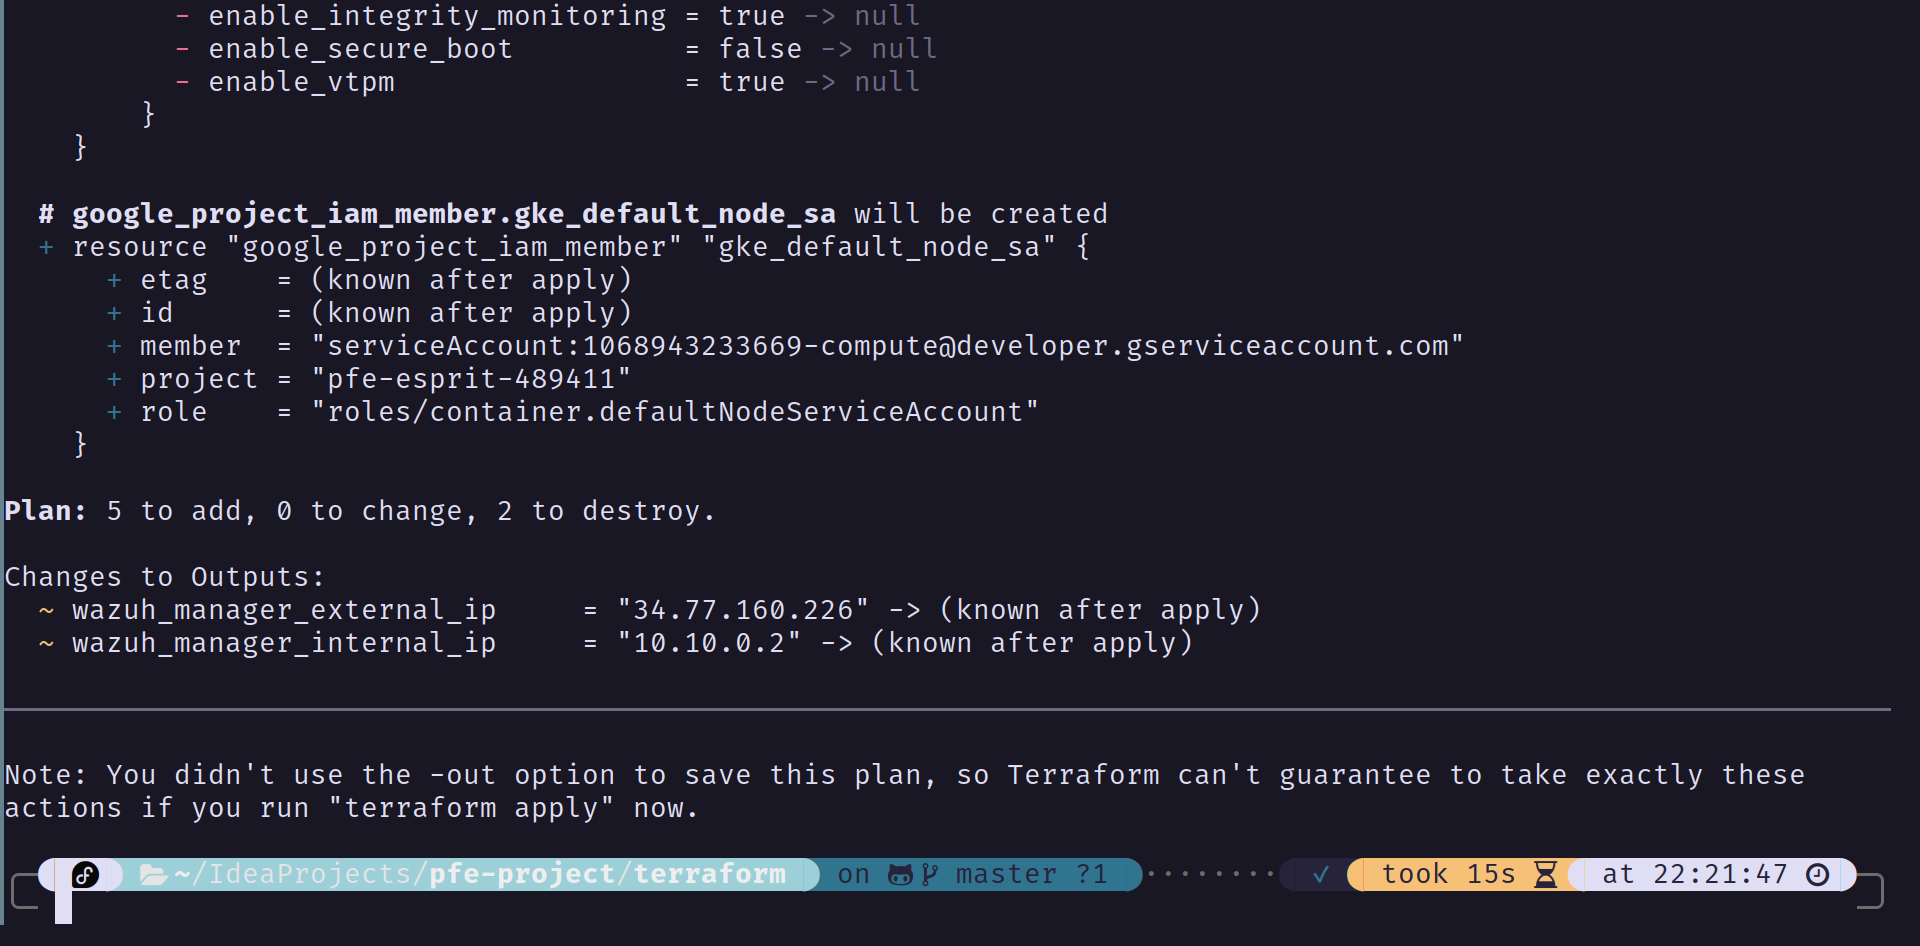
\includegraphics[width=0.95\textwidth,keepaspectratio]{images/screenshots/terraform-plan-gke-node-service-account-changes}
    \caption{Sortie de \texttt{terraform plan} montrant les changements sur le service account GKE}
    \label{fig:terraform_plan}
\end{figure}

\begin{figure}[H]
    \centering
    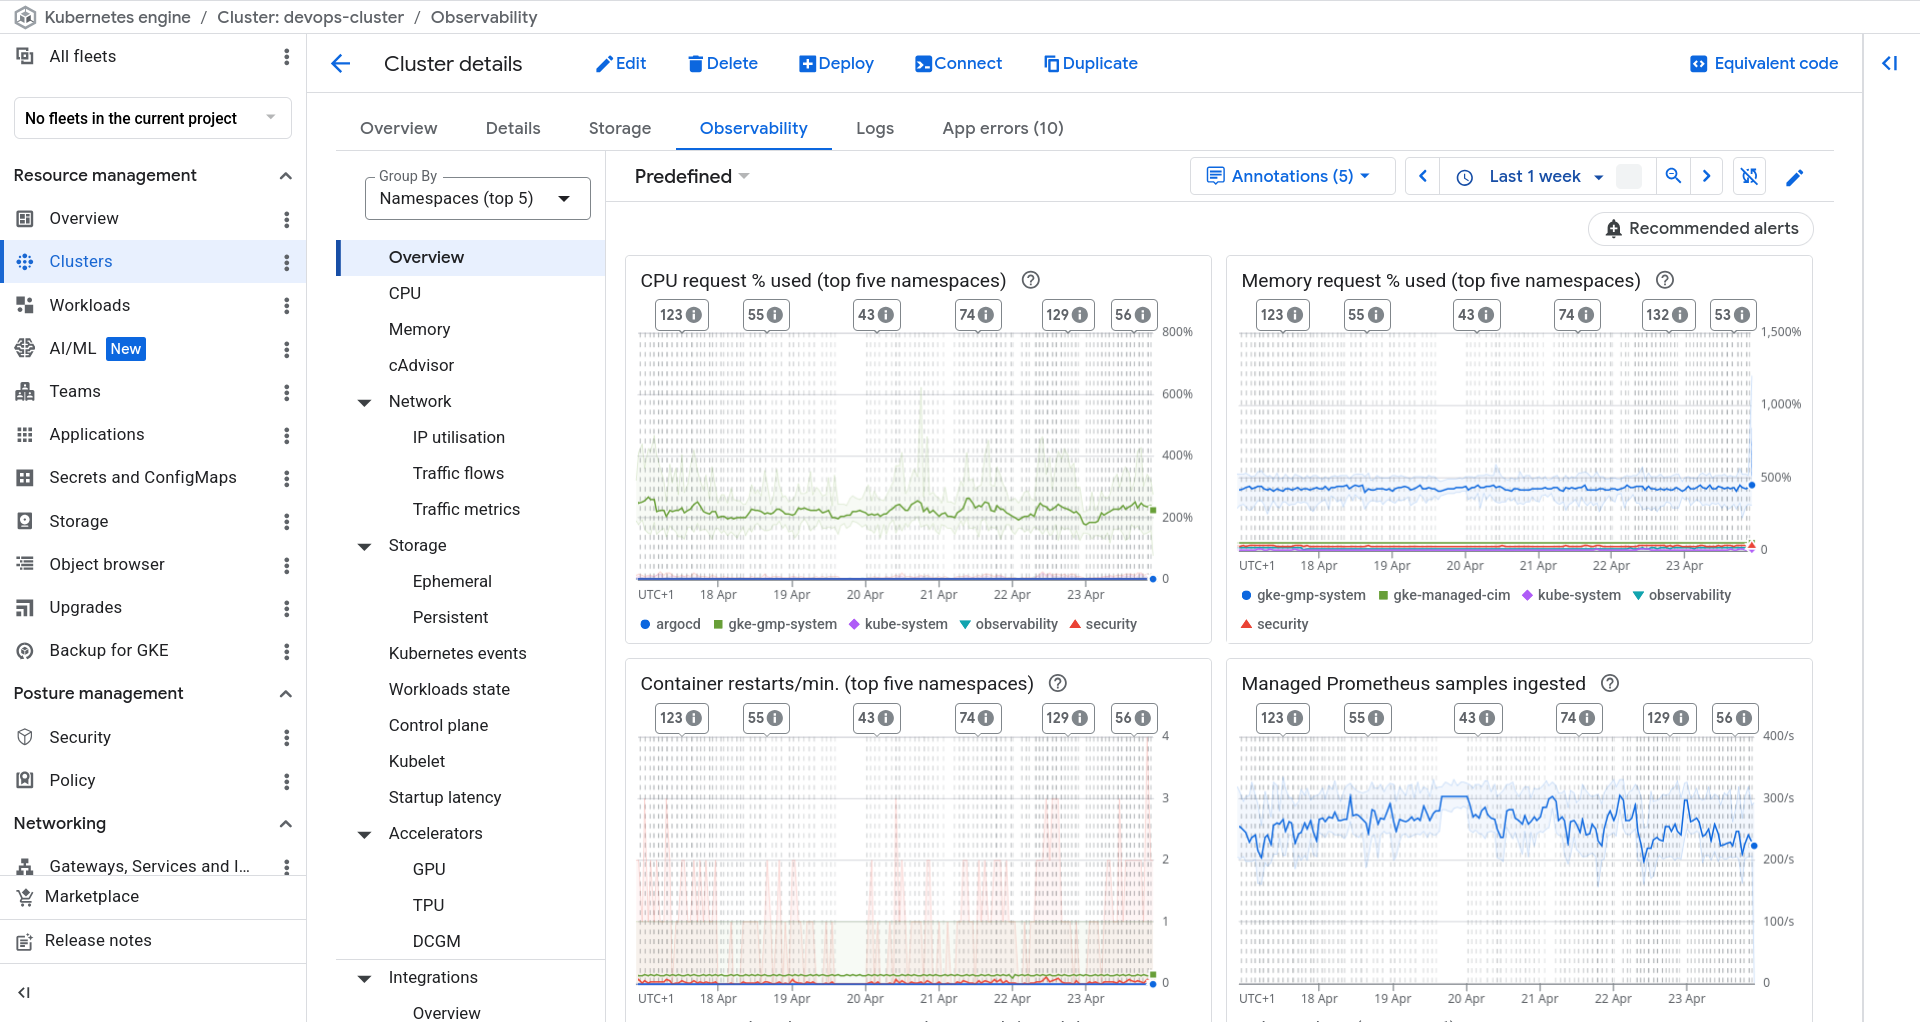
\includegraphics[width=0.95\textwidth,keepaspectratio]{images/screenshots/gke-cluster-observability-dashboard}
    \caption{Dashboard du cluster GKE Autopilot dans la console GCP}
    \label{fig:gke_console}
\end{figure}

\subsection{Rétrospective Sprint 1}

\begin{table}[H]
\centering
\setlength{\arrayrulewidth}{0.8pt}
\renewcommand{\arraystretch}{1.4}
\caption{Rétrospective Sprint 1}
\label{tab:retro_s1}
\begin{tabularx}{\textwidth}{|>{\centering\arraybackslash}X|X|}
\hline
\tableheader \textbf{Catégorie} & \textbf{Détail} \\
\hline
Ce qui a bien marché & Infrastructure 100\% reproductible, Terraform plan clair \\
\hline
Difficultés & Configuration initiale du WIF provider, activation séquentielle des APIs GCP \\
\hline
Livrable & Cluster GKE + VPC + IAM + VM Wazuh opérationnels \\
\hline
\end{tabularx}
\end{table}


%% ================================================================
%%  SPRINT 2 — Containerisation et Pipeline CI/CD
%% ================================================================
\section{Sprint 2~: Containerisation et Pipeline CI/CD}

\subsection{Objectif et Backlog du Sprint}

\begin{table}[H]
\centering
\setlength{\arrayrulewidth}{0.8pt}
\setlength{\dashlinedash}{3pt}
\setlength{\dashlinegap}{2pt}
\renewcommand{\arraystretch}{1.4}
\caption{Backlog du Sprint 2}
\label{tab:backlog_s2}
\begin{tabularx}{\textwidth}{|>{\centering\arraybackslash}X|>{\centering\arraybackslash}X|>{\centering\arraybackslash}X|}
\hline
\tableheader \textbf{User Story} & \textbf{Tâche} & \textbf{Statut} \\
\hline
US-03~: Dockerfile multi-stage & Écrire le Dockerfile avec build Bun + runner Nginx & Terminé \\ \hdashline
US-03 & Introduire les vulnérabilités intentionnelles (nginx:1.21, secrets ENV) & Terminé \\ \hdashline
US-04~: Pipeline CI & Configurer GitHub Actions (build-test, app-image-release) & Terminé \\ \hdashline
US-05~: Auth Keyless (WIF) & Configurer l'authentification OIDC dans le pipeline & Terminé \\ \hdashline
US-04 & Configurer le job update-k8s-tags & Terminé \\
\hline
\end{tabularx}
\end{table}

\subsection{Containerisation et Sécurité des Images Docker}

\subsubsection{Build Multi-Étapes}

Le \texttt{Dockerfile} utilise un \textbf{build multi-étapes} pour minimiser la taille
de l'image finale et réduire la surface d'attaque~:

\begin{lstlisting}[language=bash, caption=Dockerfile multi-étapes (version vulnérable pour démo)]
# Stage 1 : Build avec Bun
FROM oven/bun:1 AS builder
WORKDIR /app
COPY package.json bun.lock ./
RUN bun install
COPY . .
RUN bun run build
# --> dist/ contient les assets statiques compiles
# Stage 2 : Serveur Nginx minimal
FROM nginx:1.21 AS runner   # Attention : version vulnerable (demo)
COPY --from=builder /app/dist /usr/share/nginx/html
COPY ./nginx.conf /etc/nginx/conf.d/default.conf
EXPOSE 80
CMD ["nginx", "-g", "daemon off;"]
\end{lstlisting}

\subsubsection{Vulnérabilités Intentionnelles dans le Dockerfile}

\begin{table}[H]
\centering
\setlength{\arrayrulewidth}{0.8pt}
\setlength{\dashlinedash}{3pt}
\setlength{\dashlinegap}{2pt}
\renewcommand{\arraystretch}{1.4}
\caption{Vulnérabilités intentionnelles dans le Dockerfile}
\label{tab:dockerfile_vulns}
\begin{tabularx}{\textwidth}{|>{\centering\arraybackslash}X|>{\centering\arraybackslash}X|>{\centering\arraybackslash}X|>{\centering\arraybackslash}X|}
\hline
\tableheader \textbf{Vulnérabilité} & \textbf{Ligne} & \textbf{Outil} & \textbf{Sévérité} \\
\hline
Image nginx obsolète (CVEs OS) & \texttt{FROM nginx:1.21} & Trivy & CRITICAL/HIGH \\ \hdashline
Secrets hardcodés en ENV & \texttt{ENV APP\_SECRET=...} & Trivy & HIGH \\ \hdashline
Fichier .env copié dans l'image & \texttt{COPY .env ...} & Trivy & HIGH \\ \hdashline
Exécution en root (pas de USER) & Absent & Trivy DS002 & MEDIUM \\ \hdashline
Pas de HEALTHCHECK & Absent & Trivy DS026 & LOW \\
\hline
\end{tabularx}
\end{table}

\subsubsection{Comparaison Image Vulnérable vs Durcie}

\begin{table}[H]
\centering
\setlength{\arrayrulewidth}{0.8pt}
\setlength{\dashlinedash}{3pt}
\setlength{\dashlinegap}{2pt}
\renewcommand{\arraystretch}{1.4}
\caption{nginx:1.21 vs nginx:alpine}
\label{tab:nginx_compare}
\begin{tabularx}{\textwidth}{|>{\centering\arraybackslash}X|>{\centering\arraybackslash}X|>{\centering\arraybackslash}X|}
\hline
\tableheader \textbf{Aspect} & \textbf{nginx:1.21 (vulnérable)} & \textbf{nginx:alpine (durci)} \\
\hline
CVEs OS critiques & Plusieurs dizaines & Quasi-inexistants \\ \hdashline
Taille image & $\sim$133 MB & $\sim$23 MB \\ \hdashline
Utilisateur & root & non-root possible \\ \hdashline
Surface d'attaque & Large & Minimale \\
\hline
\end{tabularx}
\end{table}

\subsection{Pipeline CI/CD avec GitHub Actions}

\subsubsection{Vue Globale du Pipeline}

Le pipeline GitHub Actions est déclenché à chaque \textit{push} sur la branche principale.
Il s'articule en plusieurs jobs interdépendants~:
\begin{enumerate}
  \item \textbf{build-test}~: tests unitaires, lint, SonarCloud, Trivy FS~;
  \item \textbf{prepare-release-infra}~: parallèle app-image-release et playwright-release~;
  \item \textbf{app-image-release}~: build image Docker, push vers Artifact Registry, scan Trivy~;
  \item \textbf{update-k8s-tags}~: commit du nouveau SHA dans les manifests Kubernetes~;
  \item \textbf{e2e-tests}~: matrice de 6 jobs Playwright (@t1 à @t6)~;
  \item \textbf{zap-baseline}~: scan DAST OWASP ZAP post-déploiement.
\end{enumerate}

\begin{figure}[H]
    \centering
    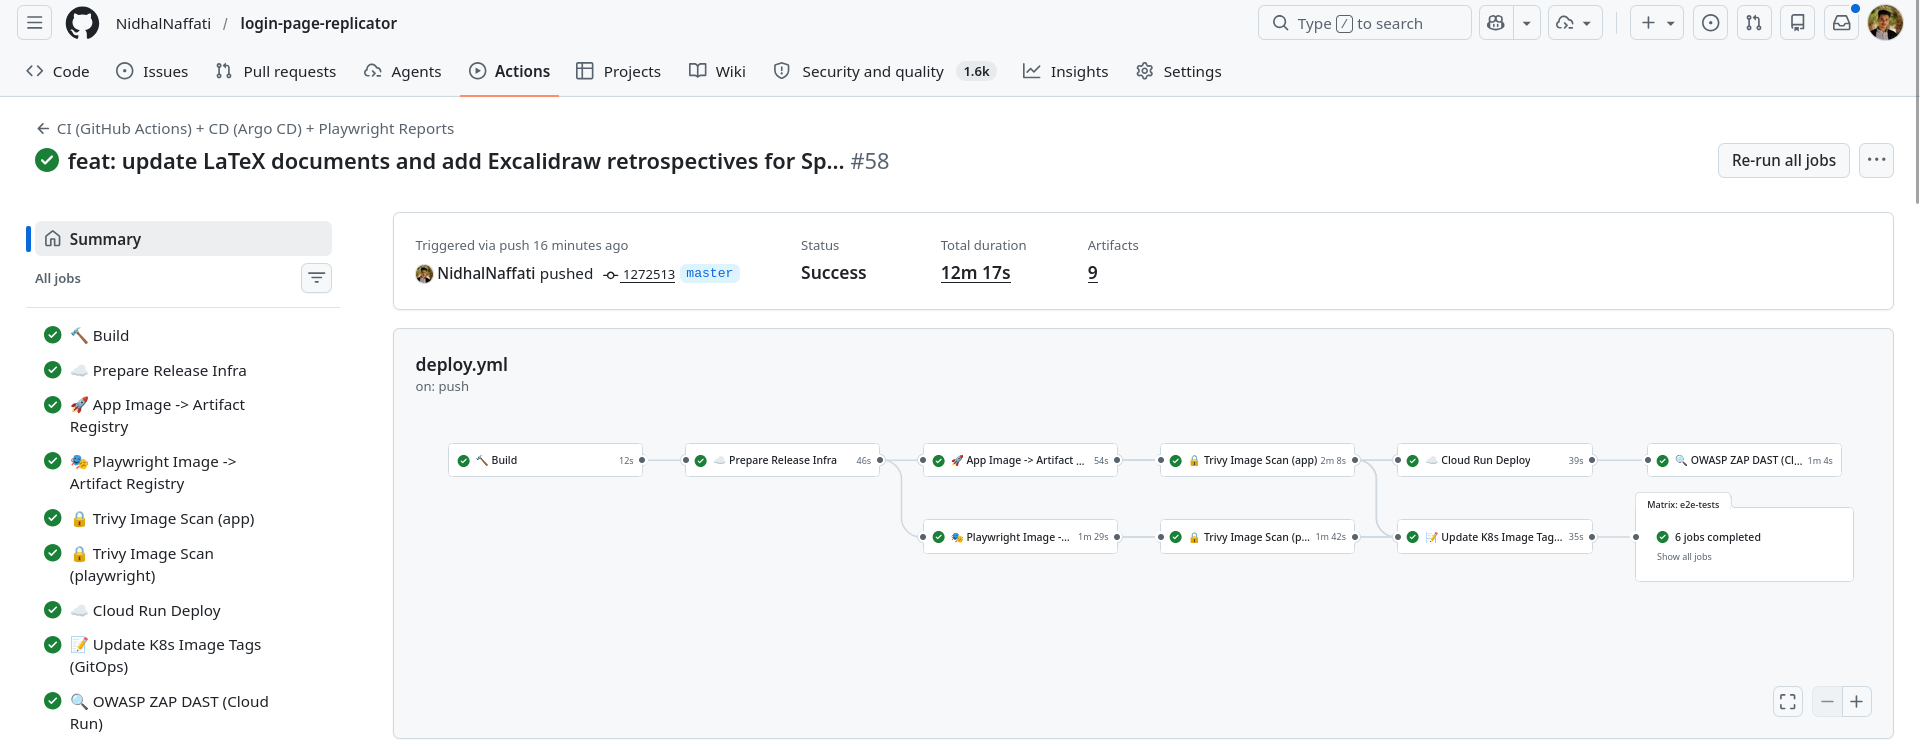
\includegraphics[width=0.95\textwidth,keepaspectratio]{images/screenshots/github-actions-ci-cd-workflow-summary}
    \caption{Vue globale du pipeline CI/CD dans GitHub Actions}
    \label{fig:pipeline_overview}
\end{figure}

\subsubsection{Job build-test --- Première Ligne de Défense}

Le job \texttt{build-test} constitue la premiere ligne de defense securitaire~:
\begin{lstlisting}[language=bash, caption=Extrait du job build-test GitHub Actions]
build-test:
  runs-on: ubuntu-latest
  steps:
    - uses: actions/checkout@v4
    - uses: oven-sh/setup-bun@v2
    - run: bun install
    - run: bun run lint
    - run: bun run test:coverage
    - name: SonarCloud Scan
      uses: SonarSource/sonarcloud-github-action@master
      env:
        SONAR_TOKEN: ${{ secrets.SONAR_TOKEN }}
    - name: Trivy FS Scan
      uses: aquasecurity/trivy-action@master
      with:
        scan-type: 'fs'
        format: 'sarif'
        output: 'trivy-fs-results.sarif'
        scanners: 'vuln,secret,misconfig'
    - uses: github/codeql-action/upload-sarif@v3
      with:
        sarif_file: 'trivy-fs-results.sarif'
\end{lstlisting}
\subsubsection{Authentification sans Clés Statiques --- Workload Identity Federation}
L'un des apports majeurs de ce projet est le remplacement des clés JSON statiques par
l'authentification \textbf{OIDC via Workload Identity Federation}~:
\begin{lstlisting}[language=bash, caption=Authentification GCP sans clé statique]
# Avant : secrets.GCP_SA_KEY (cle JSON longue duree)
# Apres :
- name: Authenticate to GCP via WIF
  uses: google-github-actions/auth@v2
  with:
    workload_identity_provider: ${{ secrets.WIF_PROVIDER }}
    service_account: ${{ secrets.WIF_SERVICE_ACCOUNT }}
\end{lstlisting}
GitHub Actions obtient un \textbf{token OIDC éphémère} valide 1 heure maximum, échangé
contre des credentials GCP temporaires. Aucune clé persistante n'est stockée.
\begin{figure}[H]
    \centering
    \fbox{\parbox{0.85\textwidth}{\centering
        \vspace{2.5cm}
        Espace réservé pour la Figure~\ref{fig:build_test_screenshot}\\
        \textbf{Capture d'écran~: Job build-test réussi dans GitHub Actions}
        \vspace{2.5cm}
    }}
    \caption{Exécution réussie du job build-test}
    \label{fig:build_test_screenshot}
\end{figure}
\subsection{Orchestration Kubernetes sur GKE}
Le déploiement définit \textbf{deux containers dans le même pod}~:
\begin{itemize}
  \item \textbf{Container \texttt{app}}~: image Nginx servant l'application React compilée,
        port 80, ressources \texttt{cpu: 100m}, \texttt{memory: 128Mi}~;
  \item \textbf{Container \texttt{nginx-exporter}} (sidecar)~: image
        \texttt{nginx/nginx-prometheus-exporter:1.1.0}, expose les métriques Nginx en format
        Prometheus sur le port 9113.
\end{itemize}
L'HPA maintient \textbf{2 replicas minimum} et scale jusqu'à \textbf{8 replicas} à 60\%
d'utilisation CPU. Un Ingress GCE expose l'application sur Internet.
\subsection{Rétrospective Sprint 2}

\begin{table}[H]
\centering
\setlength{\arrayrulewidth}{0.8pt}
\renewcommand{\arraystretch}{1.4}
\caption{Rétrospective Sprint 2}
\label{tab:retro_s2}
\begin{tabularx}{\textwidth}{|>{\centering\arraybackslash}X|X|}
\hline
\tableheader \textbf{Catégorie} & \textbf{Détail} \\
\hline
Ce qui a bien marché & Pipeline CI fonctionnel dès le premier push, WIF opérationnel \\
\hline
Difficultés & Configuration OIDC WIF (concepts peu documentés), orchestration des jobs GitHub Actions \\
\hline
Livrable & Pipeline CI/CD complet, image Docker publiée, app déployée sur GKE \\
\hline
\end{tabularx}
\end{table}


%% ================================================================
%%  SPRINT 3 — Sécurité Intégrée et GitOps
%% ================================================================
\section{Sprint 3~: Sécurité Intégrée et GitOps}

\subsection{Objectif et Backlog du Sprint}

\begin{table}[H]
\centering
\setlength{\arrayrulewidth}{0.8pt}
\setlength{\dashlinedash}{3pt}
\setlength{\dashlinegap}{2pt}
\renewcommand{\arraystretch}{1.4}
\caption{Backlog du Sprint 3}
\label{tab:backlog_s3}
\begin{tabularx}{\textwidth}{|>{\centering\arraybackslash}X|>{\centering\arraybackslash}X|>{\centering\arraybackslash}X|}
\hline
\tableheader \textbf{User Story} & \textbf{Tâche} & \textbf{Statut} \\
\hline
US-06~: Scans SAST/SCA & Intégrer SonarCloud et Trivy (3 niveaux) dans le pipeline & Terminé \\ \hdashline
US-07~: GitOps Argo CD & Configurer l'Application Argo CD avec auto-sync et self-heal & Terminé \\ \hdashline
US-07 & Configurer les PostSync hooks pour Playwright & Terminé \\ \hdashline
US-08~: Zero Trust & Créer les 12 NetworkPolicies default-deny & Terminé \\ \hdashline
US-09~: DAST ZAP & Intégrer le scan OWASP ZAP baseline post-déploiement & Terminé \\
\hline
\end{tabularx}
\end{table}

\subsection{SAST avec SonarCloud}

SonarCloud analyse le code TypeScript/React à chaque push et détecte~:
\begin{itemize}
  \item \textbf{Security Hotspots}~: utilisations de \texttt{dangerouslySetInnerHTML} (XSS)~;
  \item \textbf{Vulnerabilities}~: patterns de code pouvant mener à des injections~;
  \item \textbf{Code Smells}~: indicateurs de qualité masquant des vulnérabilités~;
  \item \textbf{Coverage gate}~: bloque la PR si la couverture de tests chute sous le seuil.
\end{itemize}

\begin{figure}[H]
    \centering
    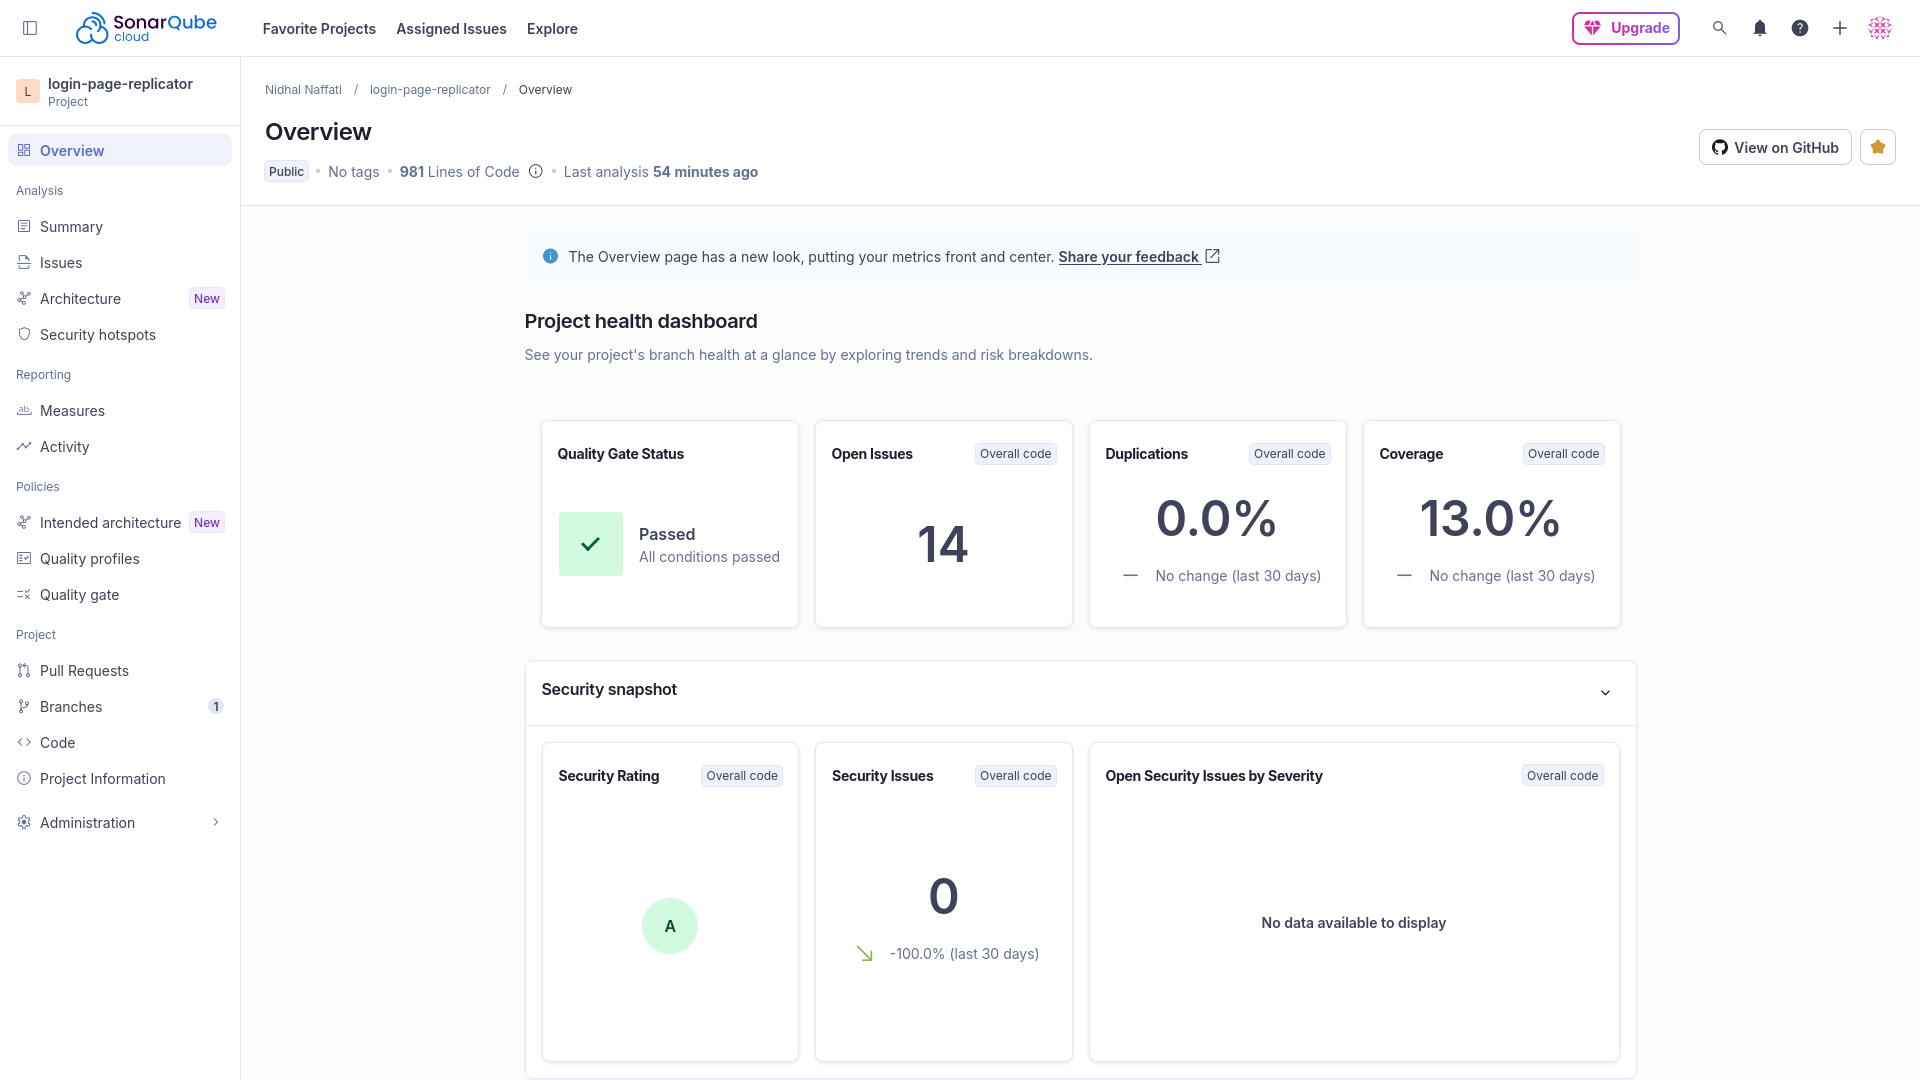
\includegraphics[width=0.95\textwidth,keepaspectratio]{images/screenshots/sonarqube-overview-dashboard}
    \caption{Dashboard SonarCloud montrant la vue d'ensemble du projet}
    \label{fig:sonarcloud_dashboard}
\end{figure}

\begin{figure}[H]
    \centering
    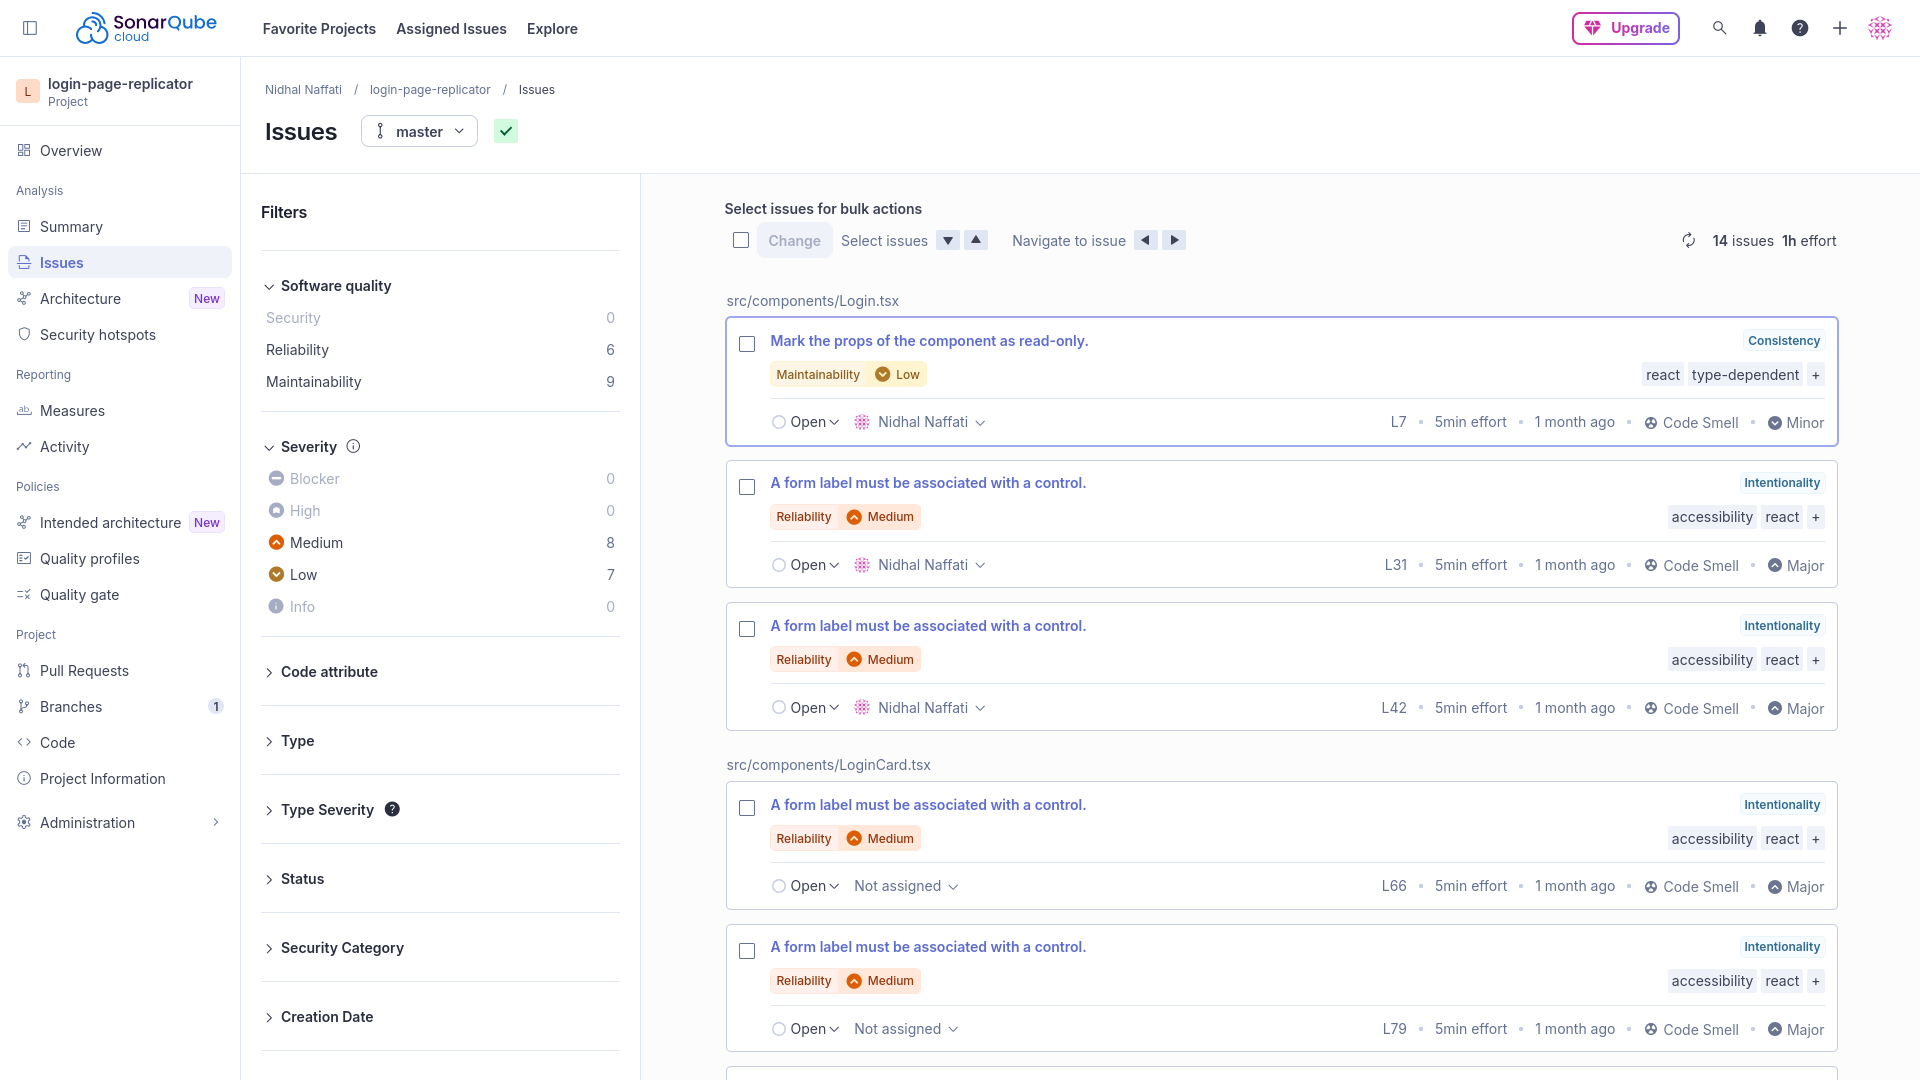
\includegraphics[width=0.95\textwidth,keepaspectratio]{images/screenshots/sonarqube-issues-list}
    \caption{Liste des issues de sécurité détectées par SonarCloud}
    \label{fig:sonarcloud_issues}
\end{figure}

\subsection{SCA avec Trivy --- Vulnérabilités Détectées}

Le tableau~\ref{tab:trivy_scans} détaille les trois niveaux de scan Trivy intégrés~:

\begin{table}[H]
\centering
\setlength{\arrayrulewidth}{0.8pt}
\setlength{\dashlinedash}{3pt}
\setlength{\dashlinegap}{2pt}
\renewcommand{\arraystretch}{1.4}
\caption{Les trois niveaux de scan Trivy dans le pipeline}
\label{tab:trivy_scans}
\begin{tabularx}{\textwidth}{|>{\centering\arraybackslash}X|>{\centering\arraybackslash}X|>{\centering\arraybackslash}X|}
\hline
\tableheader \textbf{Scan} & \textbf{Cible} & \textbf{Ce qui est détecté} \\
\hline
\texttt{trivy fs} & Code source + \texttt{package.json} & Vulns deps npm, secrets dans fichiers \\ \hdashline
\texttt{trivy image} & Image Docker construite & CVEs OS, secrets ENV \\ \hdashline
\texttt{trivy config} & Manifests YAML Kubernetes & Misconfigurations IaC \\
\hline
\end{tabularx}
\end{table}

\begin{table}[H]
\centering
\setlength{\arrayrulewidth}{0.8pt}
\setlength{\dashlinedash}{3pt}
\setlength{\dashlinegap}{2pt}
\renewcommand{\arraystretch}{1.4}
\caption{CVEs détectées par Trivy FS sur les dépendances npm}
\label{tab:cves_npm}
\begin{tabularx}{\textwidth}{|>{\centering\arraybackslash}X|>{\centering\arraybackslash}X|>{\centering\arraybackslash}X|>{\centering\arraybackslash}X|}
\hline
\tableheader \textbf{CVE} & \textbf{Package} & \textbf{Sévérité} & \textbf{Description} \\
\hline
CVE-2021-23337 & lodash 4.17.20 & HIGH & Command Injection \\ \hdashline
CVE-2026-4800  & lodash 4.17.20 & HIGH & Code Injection via \_.template \\ \hdashline
CVE-2025-13465 & lodash 4.17.20 & MEDIUM & Prototype Pollution \\ \hdashline
CVE-2022-23539 & jsonwebtoken 8.5.1 & HIGH & Insecure key types \\ \hdashline
CVE-2022-23540 & jsonwebtoken 8.5.1 & MEDIUM & Signature bypass (none algo) \\ \hdashline
CVE-2022-23541 & jsonwebtoken 8.5.1 & MEDIUM & RSA to HMAC forgery \\ \hdashline
CVE-2024-29041 & express 4.17.1 & MEDIUM & Open Redirect \\
\hline
\end{tabularx}
\end{table}

Le scan de l'image \texttt{nginx:1.21} révèle \textbf{47 vulnérabilités}~: 3 CRITICAL, 12 HIGH,
18 MEDIUM, 14 LOW.

\begin{figure}[H]
    \centering
    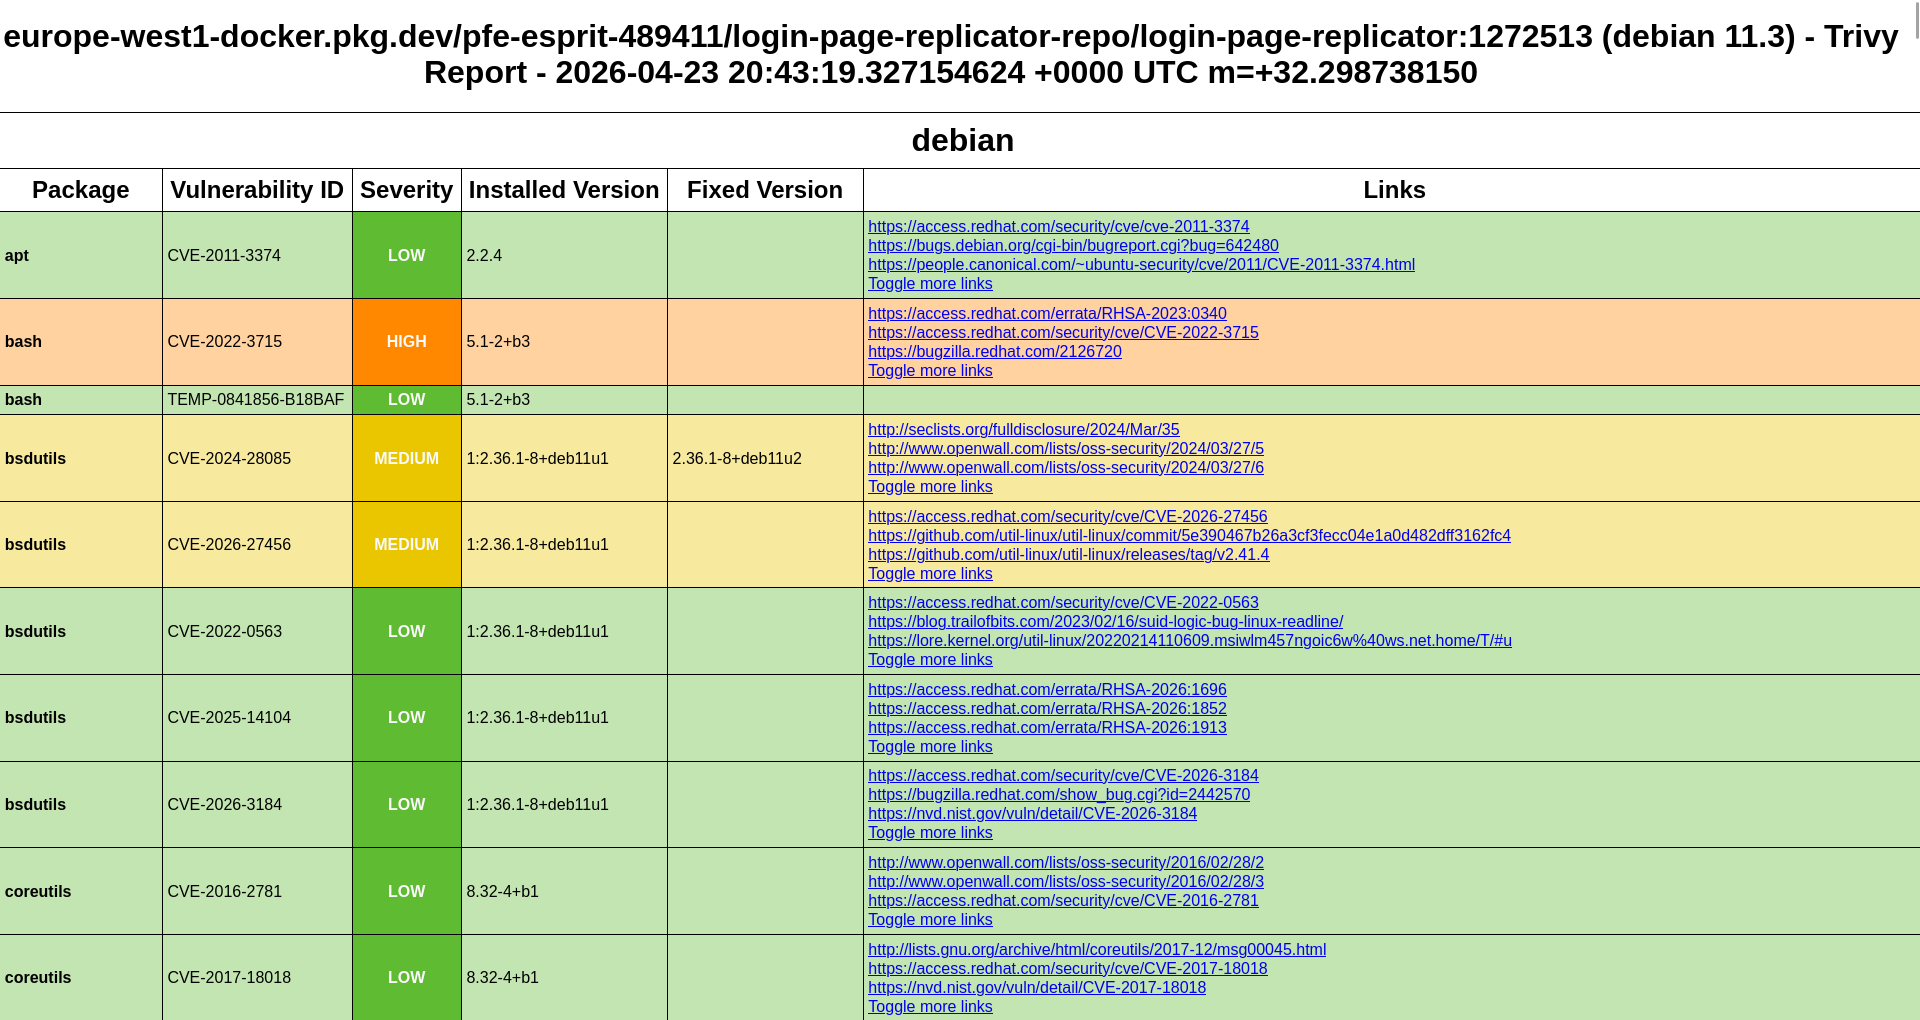
\includegraphics[width=0.95\textwidth,keepaspectratio]{images/screenshots/trivy-debian-vulnerability-report-overview}
    \caption{Vue d'ensemble du rapport Trivy sur l'image nginx:1.21 (Debian)}
    \label{fig:trivy_scan_results}
\end{figure}

\begin{figure}[H]
    \centering
    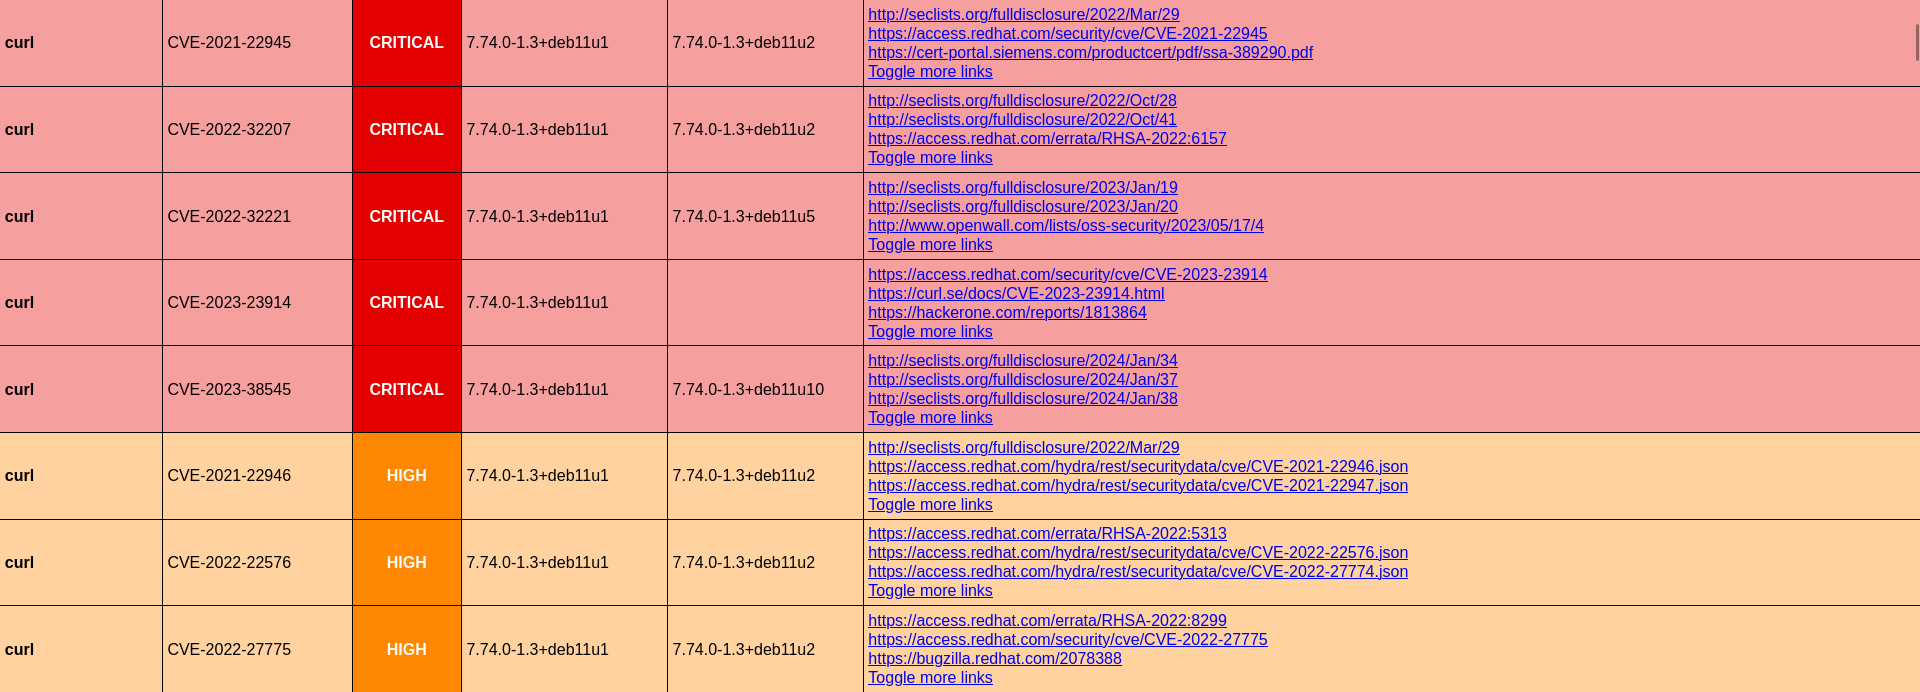
\includegraphics[width=0.95\textwidth,keepaspectratio]{images/screenshots/trivy-debian-curl-critical-vulnerabilities}
    \caption{Détail des vulnérabilités critiques détectées par Trivy (curl/libcurl)}
    \label{fig:trivy_critical_detail}
\end{figure}

\subsection{DAST avec OWASP ZAP}

OWASP ZAP effectue un scan en boîte noire de l'application déployée~:

\begin{table}[H]
\centering
\setlength{\arrayrulewidth}{0.8pt}
\setlength{\dashlinedash}{3pt}
\setlength{\dashlinegap}{2pt}
\renewcommand{\arraystretch}{1.4}
\caption{Findings OWASP ZAP sur l'application}
\label{tab:zap_findings}
\begin{tabularx}{\textwidth}{|>{\centering\arraybackslash}X|>{\centering\arraybackslash}X|>{\centering\arraybackslash}X|}
\hline
\tableheader \textbf{Finding} & \textbf{Règle} & \textbf{Sévérité} \\
\hline
Stored XSS (dangerouslySetInnerHTML) & 40012 & HIGH \\ \hdashline
Missing Content-Security-Policy & 10038 & MEDIUM \\ \hdashline
Missing X-Frame-Options (Clickjacking) & 10020 & MEDIUM \\ \hdashline
Directory Browsing Enabled & 10033 & MEDIUM \\ \hdashline
Cookie sans flag Secure & 10011 & LOW \\ \hdashline
Cookie sans flag HttpOnly & 10010 & LOW \\ \hdashline
CORS Wildcard (*) & --- & LOW \\ \hdashline
Server Version Leaked (nginx/1.21.6) & 10036 & LOW \\ \hdashline
Missing HSTS & 10035 & LOW \\ \hdashline
Missing X-Content-Type-Options & 10021 & LOW \\
\hline
\end{tabularx}
\end{table}

Après durcissement de \texttt{nginx.conf} (ajout des headers de sécurité, désactivation de
\texttt{server\_tokens} et \texttt{autoindex})~: \textbf{0 FAIL, 0 WARN}.

\subsubsection{Comparaison nginx.conf Vulnérable vs Durci}

\begin{table}[H]
\centering
\setlength{\arrayrulewidth}{0.8pt}
\setlength{\dashlinedash}{3pt}
\setlength{\dashlinegap}{2pt}
\renewcommand{\arraystretch}{1.4}
\caption{Comparaison de la configuration nginx avant et après durcissement}
\label{tab:nginx_harden}
\begin{tabularx}{\textwidth}{|>{\centering\arraybackslash}X|>{\centering\arraybackslash}X|>{\centering\arraybackslash}X|}
\hline
\tableheader \textbf{Directive} & \textbf{Vulnérable} & \textbf{Durci} \\
\hline
\texttt{server\_tokens} & \texttt{on} & \texttt{off} \\ \hdashline
\texttt{X-Powered-By} & \texttt{Nginx/1.21 + React 18} & Absent \\ \hdashline
\texttt{Content-Security-Policy} & Absent & \texttt{default-src 'self'} \\ \hdashline
\texttt{X-Frame-Options} & Absent & \texttt{DENY} \\ \hdashline
\texttt{X-Content-Type-Options} & Absent & \texttt{nosniff} \\ \hdashline
\texttt{Strict-Transport-Security} & Absent & \texttt{max-age=31536000} \\ \hdashline
\texttt{autoindex} & \texttt{on} & \texttt{off} \\ \hdashline
\texttt{Access-Control-Allow-Origin} & \texttt{*} & Absent ou domaine spécifique \\ \hdashline
\texttt{Set-Cookie} flags & Aucun flag & \texttt{Secure; HttpOnly; SameSite=Strict} \\
\hline
\end{tabularx}
\end{table}

\subsubsection{Démonstration des Vulnérabilités Applicatives}

Pour démontrer la pertinence des scanners, l'application contient des \textbf{vulnérabilités
intentionnelles clairement documentées}. Le tableau~\ref{tab:vuln_demo} synthétise les
principales démonstrations réalisables~:

\begin{table}[H]
\centering
\setlength{\arrayrulewidth}{0.8pt}
\setlength{\dashlinedash}{3pt}
\setlength{\dashlinegap}{2pt}
\renewcommand{\arraystretch}{1.4}
\caption{Démonstration des vulnérabilités détectées par les scanners}
\label{tab:vuln_demo}
\begin{tabularx}{\textwidth}{|>{\centering\arraybackslash}X|>{\centering\arraybackslash}X|>{\centering\arraybackslash}X|>{\centering\arraybackslash}X|}
\hline
\tableheader \textbf{Vulnérabilité} & \textbf{CWE} & \textbf{Fichier} & \textbf{Scanner} \\
\hline
XSS stocké (\texttt{dangerouslySetInnerHTML}) & CWE-79 & TodoItem.tsx & SonarCloud + ZAP \\ \hdashline
Open Redirect (\texttt{?redirect=}) & CWE-601 & Login.tsx & SonarCloud \\ \hdashline
Énumération d'utilisateurs & CWE-209 & Login.tsx & SonarCloud \\ \hdashline
Mode debug exposant les credentials & CWE-215 & Login.tsx & SonarCloud \\ \hdashline
Credentials hardcodés (5+ fichiers) & CWE-798 & Multiple & SonarCloud + Trivy \\ \hdashline
Cookies sans Secure/HttpOnly & CWE-614 & Login.tsx, nginx.conf & ZAP \\ \hdashline
\texttt{eval()} injection de code & CWE-95 & TodoDashboard.tsx & SonarCloud \\ \hdashline
Token forgeable (\texttt{Math.random}) & CWE-338 & AuthContext.tsx & SonarCloud \\ \hdashline
Reverse tabnabbing & CWE-1022 & TodoItem.tsx & SonarCloud \\ \hdashline
Données sensibles dans localStorage & CWE-312 & AuthContext.tsx & SonarCloud \\ \hdashline
Credentials loggés en console & CWE-532 & Login.tsx & SonarCloud \\ \hdashline
Duplication de code ($>$5\%) & CWE-1041 & helpers.ts & SonarCloud \\
\hline
\end{tabularx}
\end{table}

\textbf{Exemple de démonstration XSS~:} L'utilisateur saisit
\texttt{<img src=x onerror=alert('XSS')>} comme texte de tâche. Le composant
\texttt{TodoItem} rend ce texte via \texttt{dangerouslySetInnerHTML}, ce qui exécute
le JavaScript et affiche une boîte d'alerte. Cette vulnérabilité est détectée à la fois
par SonarCloud (règle S5247) et par OWASP ZAP (règle 40012).

\begin{figure}[H]
    \centering
    \fbox{\parbox{0.85\textwidth}{\centering
        \vspace{2.5cm}
        Espace réservé pour la Figure~\ref{fig:xss_demo}\\
        \textbf{Capture d'écran~: Démonstration de la vulnérabilité XSS stockée}\\[6pt]
        \footnotesize Payload~: \texttt{<img src=x onerror=alert('XSS')>} $\to$ alert box affichée
        \vspace{2.5cm}
    }}
    \caption{Démonstration de la vulnérabilité XSS stockée dans la Todo App}
    \label{fig:xss_demo}
\end{figure}

\begin{figure}[H]
    \centering
    \fbox{\parbox{0.85\textwidth}{\centering
        \vspace{2.5cm}
        Espace réservé pour la Figure~\ref{fig:debug_mode_demo}\\
        \textbf{Capture d'écran~: Mode debug exposant les credentials (\texttt{?debug=true})}
        \vspace{2.5cm}
    }}
    \caption{Mode debug exposant les credentials de l'application (\texttt{?debug=true})}
    \label{fig:debug_mode_demo}
\end{figure}

\begin{figure}[H]
    \centering
    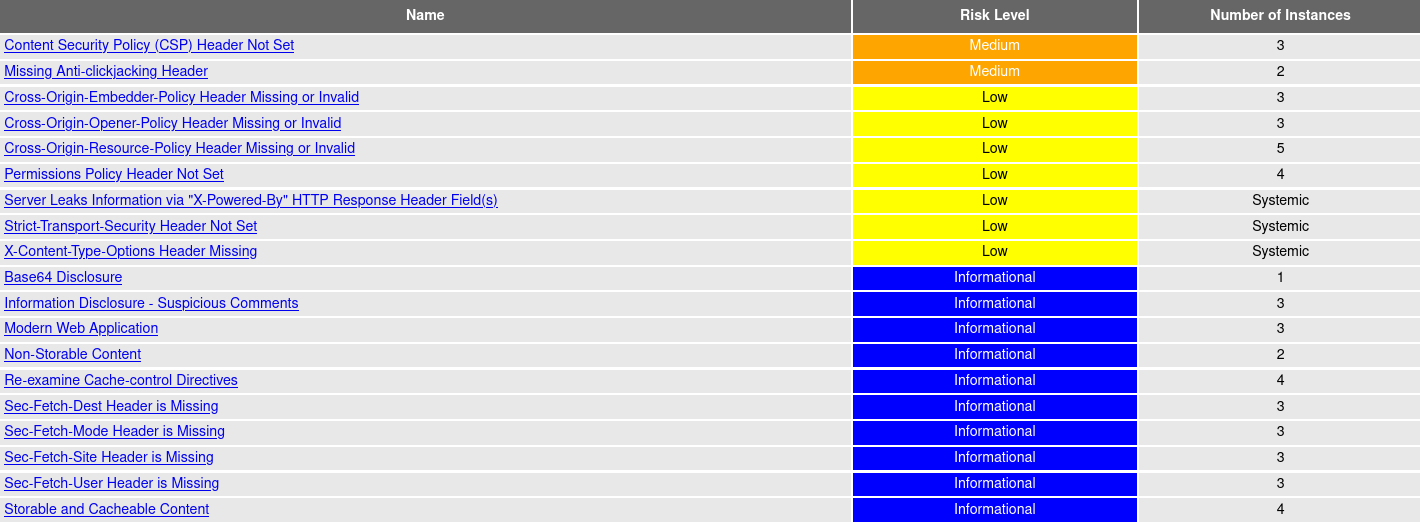
\includegraphics[width=0.95\textwidth,keepaspectratio]{images/screenshots/owasp-zap-alerts-summary}
    \caption{Résumé des alertes OWASP ZAP avant durcissement nginx}
    \label{fig:zap_report}
\end{figure}

\begin{figure}[H]
    \centering
    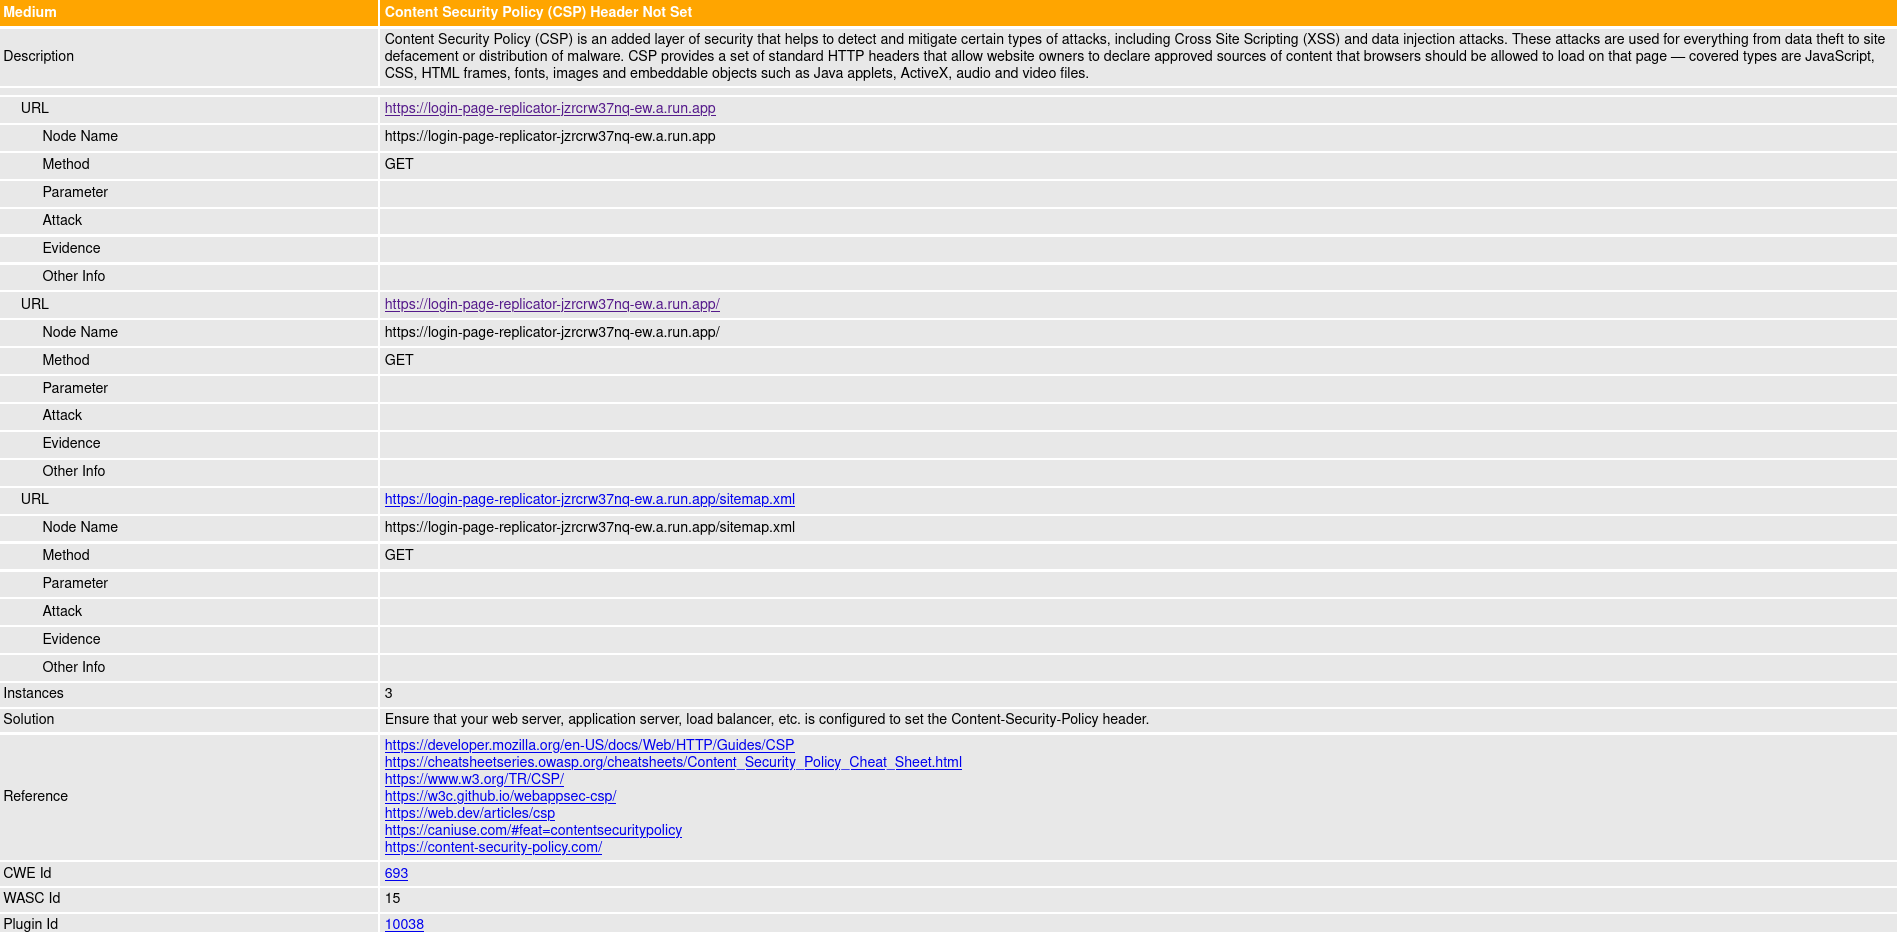
\includegraphics[width=0.95\textwidth,keepaspectratio]{images/screenshots/owasp-zap-csp-header-not-set-details}
    \caption{Détail du finding OWASP ZAP~: Content-Security-Policy header manquant}
    \label{fig:zap_csp_detail}
\end{figure}

\subsection{GitOps avec Argo CD}

\subsubsection{Configuration de l'Application Argo CD}

\begin{lstlisting}[language=bash, caption=Configuration Application Argo CD]
apiVersion: argoproj.io/v1alpha1
kind: Application
metadata:
  name: login-page-replicator
  namespace: argocd
spec:
  source:
    repoURL: https://github.com/nnaffati/login-page-replicator
    targetRevision: HEAD
    path: k8s/app
  destination:
    server: https://kubernetes.default.svc
    namespace: app
  syncPolicy:
    automated:
      prune: true     # Supprime les ressources obsoletes
      selfHeal: true  # Corrige tout drift manuel
    syncOptions:
      - CreateNamespace=true
\end{lstlisting}

\begin{figure}[H]
    \centering
    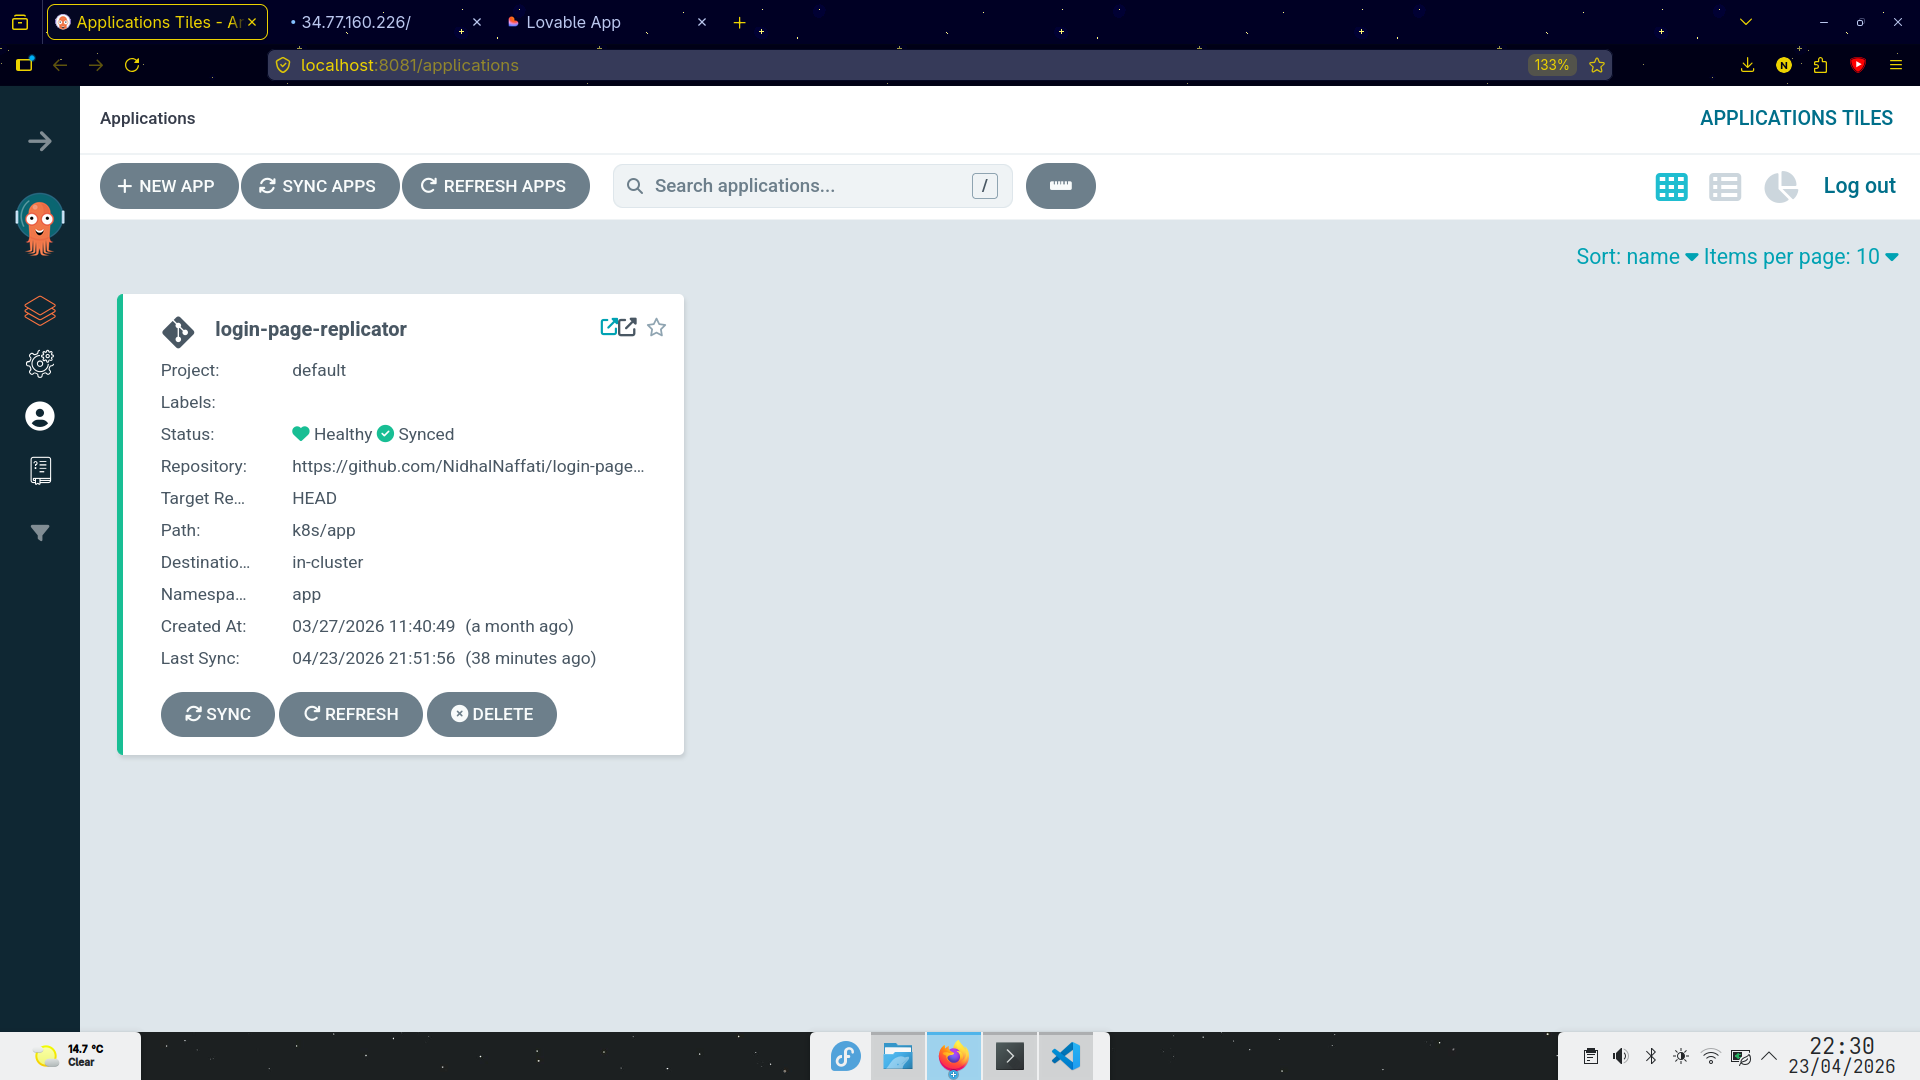
\includegraphics[width=0.95\textwidth,keepaspectratio]{images/screenshots/argocd-applications-tiles-login-page-replicator}
    \caption{Dashboard Argo CD~: vue en tuiles de l'application login-page-replicator}
    \label{fig:argocd_dashboard}
\end{figure}

\begin{figure}[H]
    \centering
    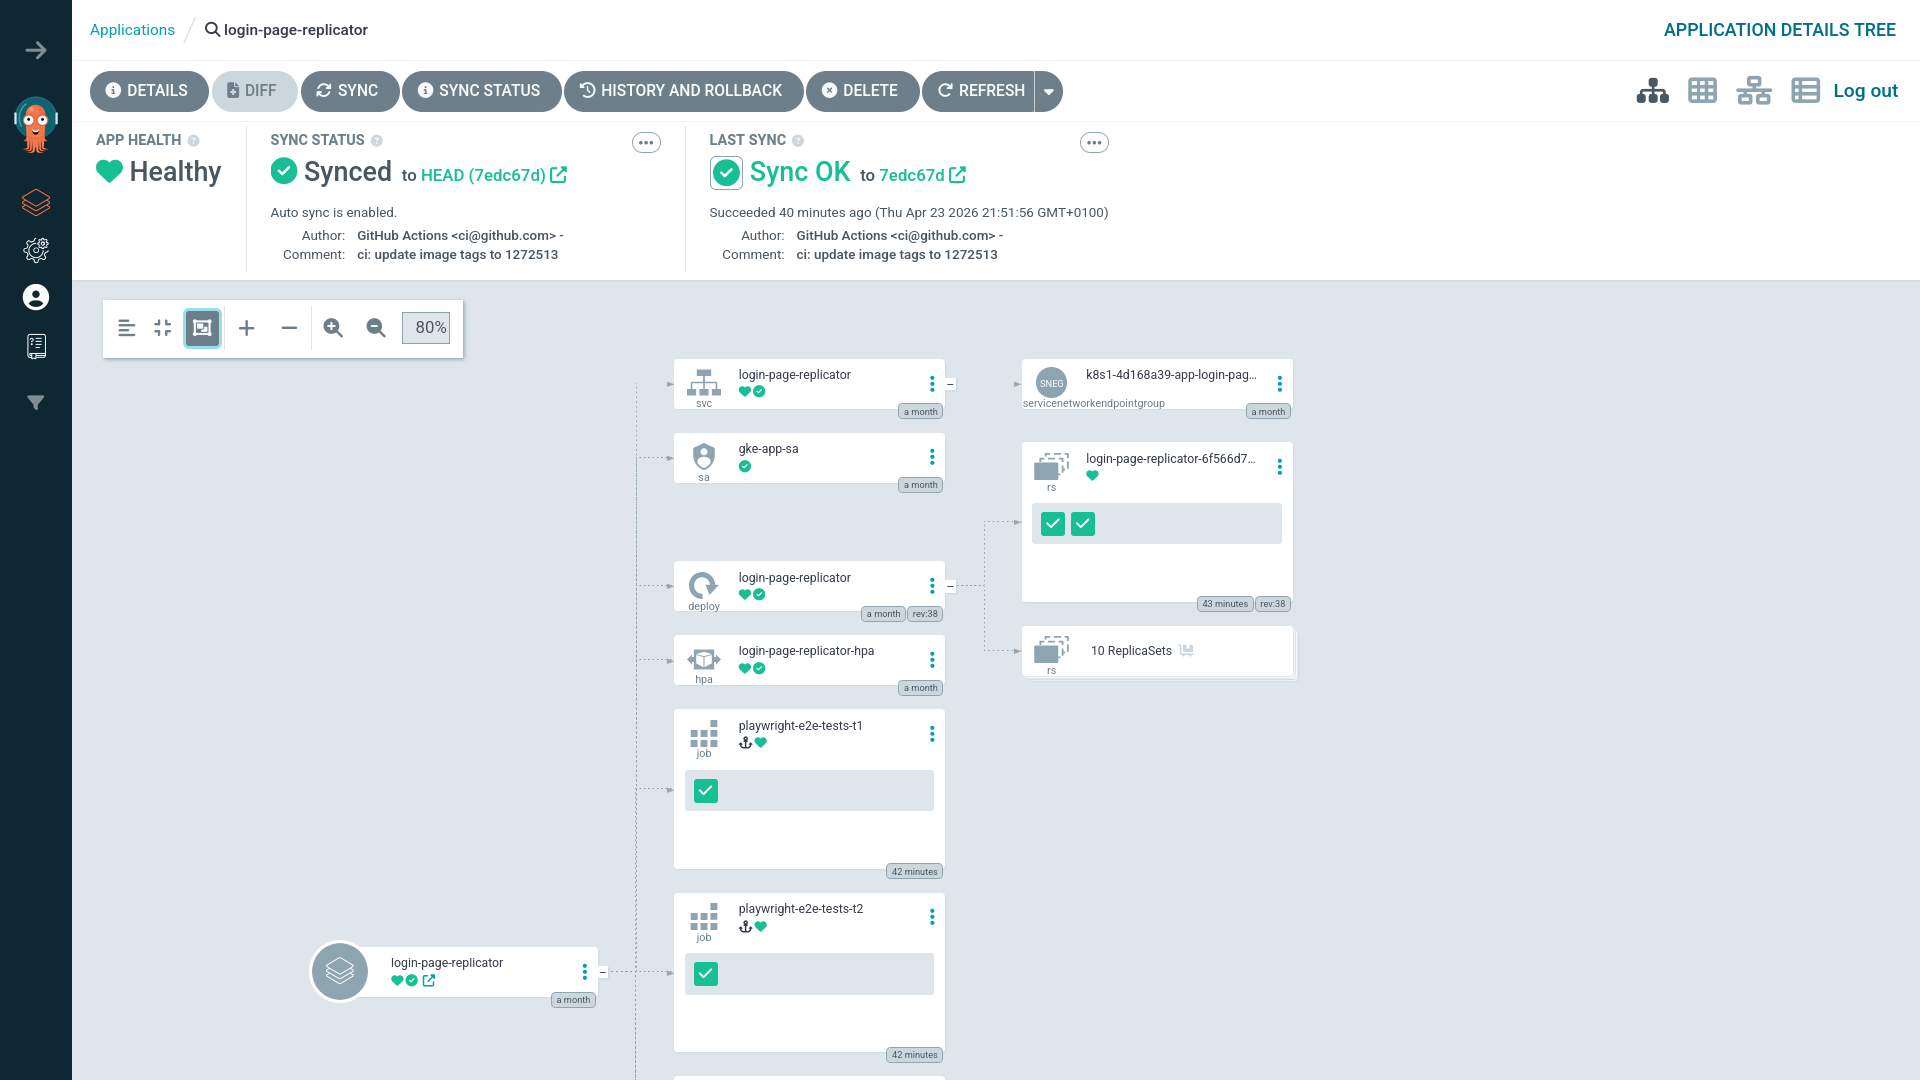
\includegraphics[width=0.95\textwidth,keepaspectratio]{images/screenshots/argocd-application-details-tree-view}
    \caption{Argo CD~: vue arborescente des ressources Kubernetes déployées}
    \label{fig:argocd_tree}
\end{figure}

\begin{figure}[H]
    \centering
    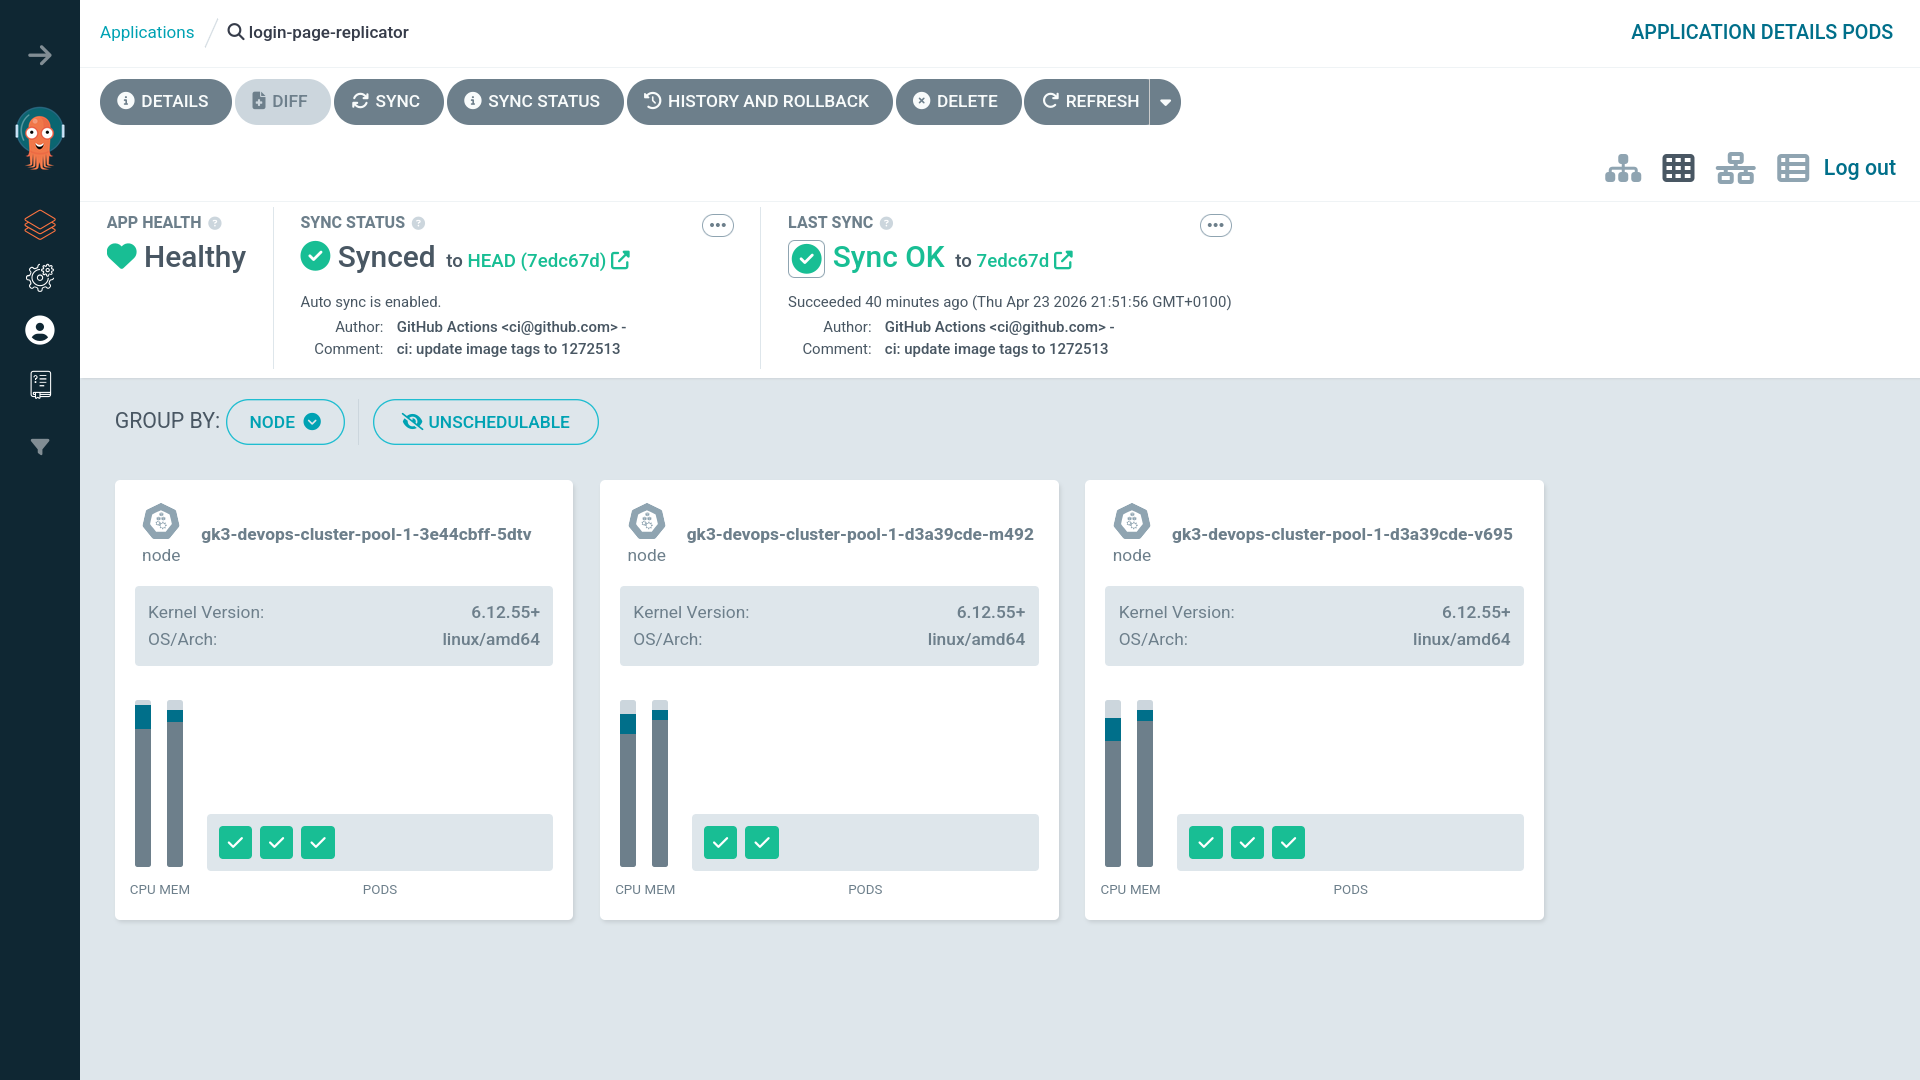
\includegraphics[width=0.95\textwidth,keepaspectratio]{images/screenshots/argocd-application-details-pods-view}
    \caption{Argo CD~: vue des pods de l'application déployée}
    \label{fig:argocd_pods}
\end{figure}

\begin{figure}[H]
    \centering
    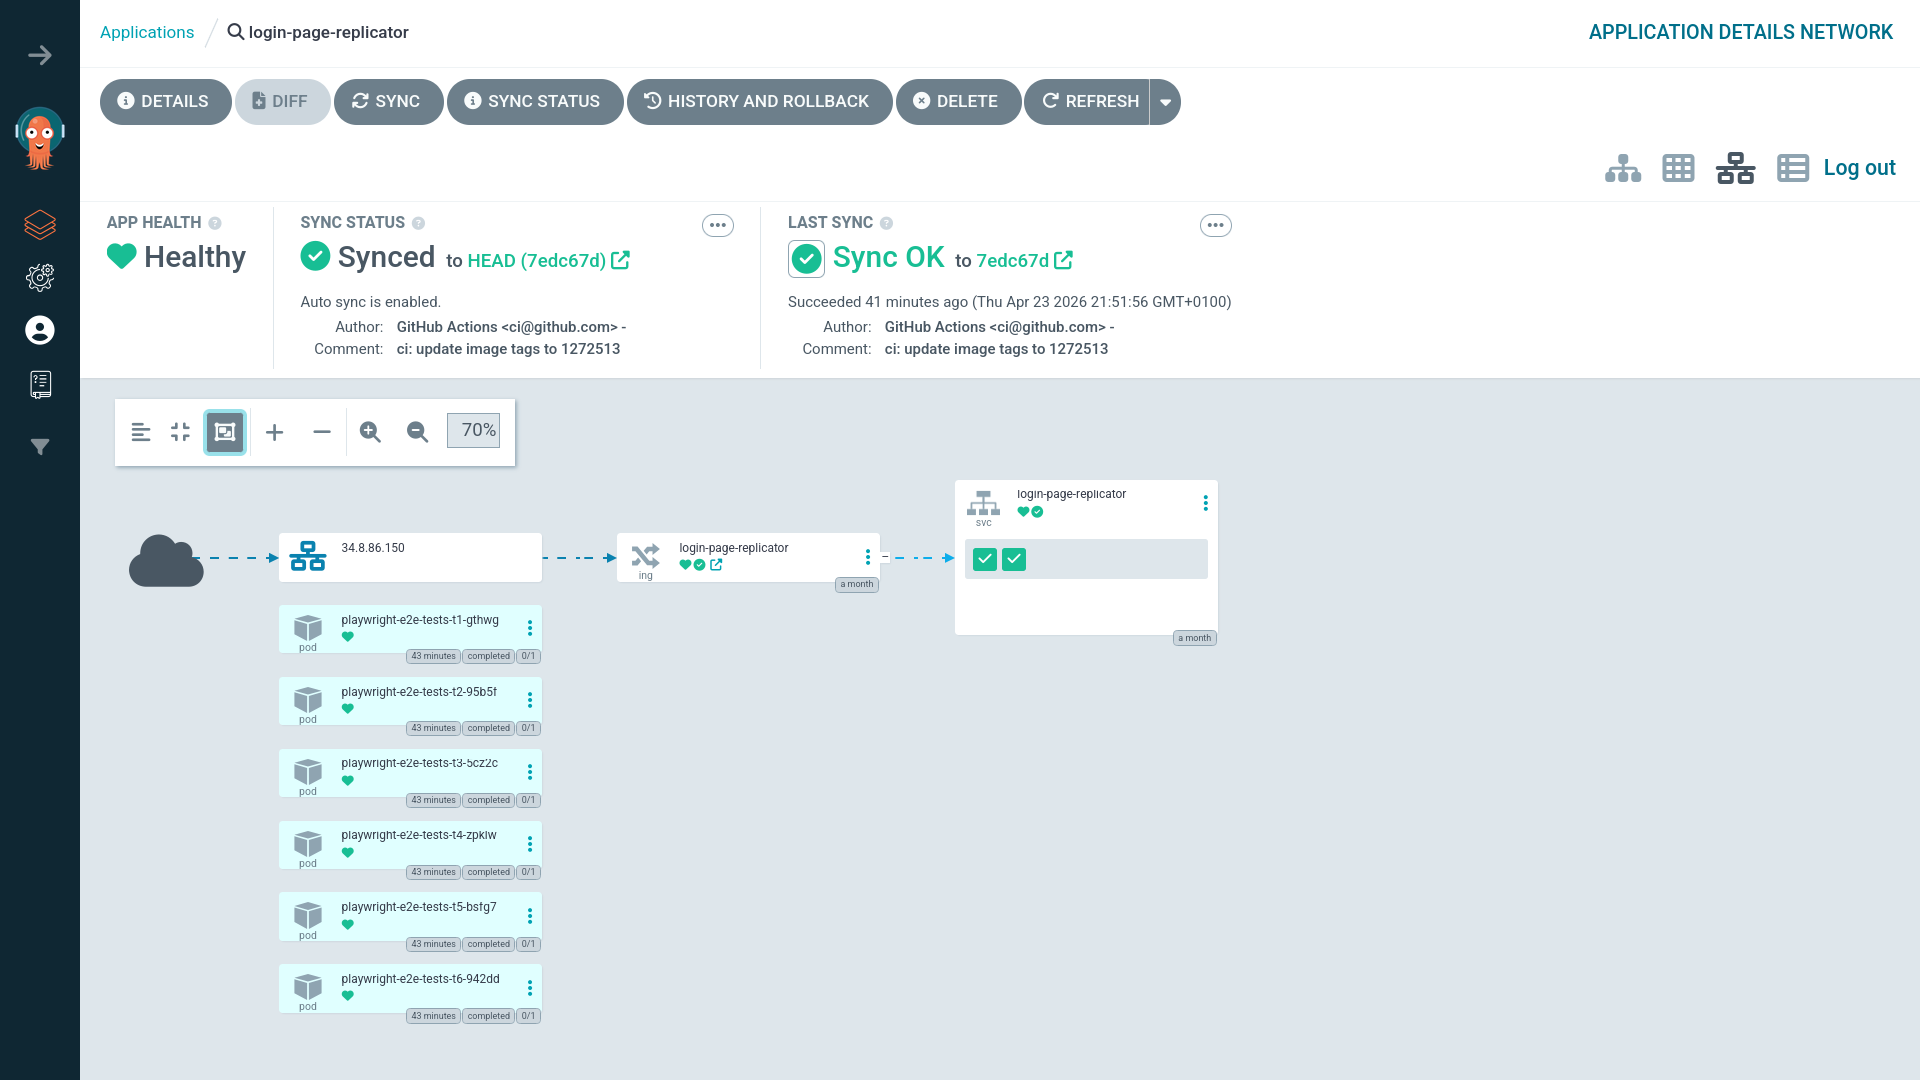
\includegraphics[width=0.95\textwidth,keepaspectratio]{images/screenshots/argocd-application-details-network-view}
    \caption{Argo CD~: vue réseau montrant les flux entre les ressources}
    \label{fig:argocd_network}
\end{figure}

\subsection{Réseau Zero Trust --- NetworkPolicies}

Le projet applique un modèle de \textbf{défense en profondeur} (\textit{Defense in Depth})
superposant plusieurs couches de contrôles indépendantes~:

\begin{table}[H]
\centering
\setlength{\arrayrulewidth}{0.8pt}
\setlength{\dashlinedash}{3pt}
\setlength{\dashlinegap}{2pt}
\renewcommand{\arraystretch}{1.4}
\caption{Modèle de défense en profondeur appliqué au projet}
\label{tab:defense_profondeur}
\begin{tabularx}{\textwidth}{|>{\centering\arraybackslash}X|>{\centering\arraybackslash}X|>{\centering\arraybackslash}X|}
\hline
\tableheader \textbf{Couche} & \textbf{Mécanisme} & \textbf{Portée} \\
\hline
L3/L4~: Périmètre GCP & Pare-feu VPC (Firewall Rules) & Filtrage source/destination entre VM/sous-réseaux \\ \hdashline
L3/L4~: Intra-cluster & NetworkPolicies Kubernetes & Filtrage pod-à-pod, namespace-à-namespace \\ \hdashline
L7~: Admission & Pod Security Standards (GKE Autopilot) & Rejet des manifests non conformes \\ \hdashline
L7~: Application & Headers HTTP durcis (nginx.conf) & Protection navigateur (CSP, HSTS, X-Frame) \\ \hdashline
Identité & Workload Identity Federation + KSA/GSA & Authentification sans clé persistante \\ \hdashline
Détection & Wazuh SIEM + Prometheus alertes & Corrélation logs, détection anomalies \\ \hdashline
Supply Chain & Trivy SCA + Image Scan + Secrets Scan & Analyse avant déploiement \\
\hline
\end{tabularx}
\end{table}

La figure~\ref{fig:defense_profondeur} illustre visuellement l'emboîtement de ces sept couches
de sécurité autour de l'application déployée.

\begin{figure}[H]
    \centering
    \includegraphics[width=0.95\textwidth,keepaspectratio]{images/defense-en-profondeur}
    \caption{Modèle de défense en profondeur --- 7 couches de sécurité}
    \label{fig:defense_profondeur}
\end{figure}

\subsubsection{Principe Default-Deny}

Sans NetworkPolicies, tous les pods communiquent librement. La politique appliquée~:
\textbf{tout est interdit par défaut, chaque flux autorisé est déclaré explicitement}.
Une politique \texttt{default-deny-all} est appliquée dans les quatre namespaces
(\texttt{app}, \texttt{testing}, \texttt{observability}, \texttt{security})~:

\begin{lstlisting}[language=bash, caption=Politique default-deny appliquée à chaque namespace]
apiVersion: networking.k8s.io/v1
kind: NetworkPolicy
metadata:
  name: default-deny-all
  namespace: app    # Replique pour: testing, observability, security
spec:
  podSelector: {}   # Selectionne TOUS les pods du namespace
  policyTypes:
    - Ingress       # Bloque tout trafic entrant
    - Egress        # Bloque tout trafic sortant
\end{lstlisting}

Sans exception explicite, aucun pod ne peut communiquer avec un autre, ni résoudre un nom
DNS, ni recevoir de health check. Chaque flux légitime est déclaré via une NetworkPolicy dédiée.

\subsubsection{Inventaire Complet des NetworkPolicies}

Le projet déploie \textbf{12 NetworkPolicies} organisées par responsabilité~:

\begin{table}[H]
\centering
\setlength{\arrayrulewidth}{0.8pt}
\setlength{\dashlinedash}{3pt}
\setlength{\dashlinegap}{2pt}
\renewcommand{\arraystretch}{1.4}
\caption{Inventaire complet des 12 NetworkPolicies déployées}
\label{tab:netpol_inventory}
\begin{tabularx}{\textwidth}{|>{\centering\arraybackslash}X|>{\centering\arraybackslash}X|>{\centering\arraybackslash}X|}
\hline
\tableheader \textbf{Politique} & \textbf{Namespace(s)} & \textbf{Rôle} \\
\hline
default-deny-all & app, testing, observability, security & Bloque tout ingress + egress \\ \hdashline
allow-dns-egress & app, testing, observability, security & Autorise UDP/TCP 53 (CoreDNS) \\ \hdashline
allow-kubelet-probes-app & app & Probes depuis nœuds + GCP LB \\ \hdashline
allow-kubelet-probes & observability & Probes sur ports 3000, 8080, 8081, 9090 \\ \hdashline
allow-prometheus-scrape & app (ingress) & Scrape depuis ns observability sur 9113 \\ \hdashline
allow-observability-to-app-metrics & observability (egress) & Egress vers app:9113 \\ \hdashline
allow-observability-internal & observability & Pod-à-pod interne \\ \hdashline
allow-apiserver-egress & observability & Egress HTTPS/443 vers API server K8s \\ \hdashline
allow-testing-to-app-http & testing + app & Tests E2E vers app sur TCP 80 \\ \hdashline
allow-playwright-hook-egress & app (egress hook) & Hook PostSync vers app:80 \\ \hdashline
allow-playwright-hook-to-app & app (ingress) & App accepte trafic du hook \\ \hdashline
allow-wazuh-agent-egress & security & Agent $\to$ Manager 10.10.0.2 sur TCP 1514/1515 \\
\hline
\end{tabularx}
\end{table}

\subsubsection{Matrice des Flux Autorisés}

\begin{table}[H]
\centering
\setlength{\arrayrulewidth}{0.8pt}
\setlength{\dashlinedash}{3pt}
\setlength{\dashlinegap}{2pt}
\renewcommand{\arraystretch}{1.4}
\caption{Matrice des flux réseau autorisés}
\label{tab:network_matrix}
\begin{tabularx}{\textwidth}{|>{\centering\arraybackslash}X|>{\centering\arraybackslash}X|>{\centering\arraybackslash}X|>{\centering\arraybackslash}X|}
\hline
\tableheader \textbf{Source} & \textbf{Destination} & \textbf{Port} & \textbf{Politique} \\
\hline
\texttt{testing} pods & \texttt{app} pods & TCP 80 & allow-testing-to-app \\ \hdashline
PostSync hook & \texttt{app} pods & TCP 80 & allow-playwright-hook \\ \hdashline
\texttt{observability} & \texttt{app} sidecar & TCP 9113 & allow-prometheus-scrape \\ \hdashline
\texttt{observability} pods & \texttt{observability} pods & Tous & allow-observability-internal \\ \hdashline
\texttt{observability} pods & API Server K8s & TCP 443 & allow-apiserver-egress \\ \hdashline
\texttt{security} DaemonSet & Wazuh VM (10.10.0.2) & TCP 1514/1515 & allow-wazuh-egress \\ \hdashline
Tous les pods & kube-dns (CoreDNS) & UDP/TCP 53 & allow-dns-egress \\ \hdashline
Nœuds (10.10.0.0/20) & \texttt{app} pods & TCP 80, 9113 & allow-kubelet-probes-app \\ \hdashline
GCP LB (130.211.0.0/22, 35.191.0.0/16) & \texttt{app} pods & TCP 80, 9113 & allow-kubelet-probes-app \\
\hline
\end{tabularx}
\end{table}

La figure~\ref{fig:network_zero_trust} fournit une vue d'ensemble des flux autorisés entre les
différents namespaces, le DNS, les nœuds (kubelet) et la VM Wazuh.

\begin{figure}[H]
    \centering
    \includegraphics[width=0.95\textwidth,keepaspectratio]{images/network-zero-trust}
    \caption{Topologie Zero Trust --- flux autorisés entre namespaces et composants externes}
    \label{fig:network_zero_trust}
\end{figure}

\subsubsection{Exemples de Politiques Cross-Namespace}

\begin{lstlisting}[language=bash, caption=allow-prometheus-scrape~: cross-namespace ingress]
apiVersion: networking.k8s.io/v1
kind: NetworkPolicy
metadata:
  name: allow-prometheus-scrape
  namespace: app
spec:
  podSelector: {}
  policyTypes:
    - Ingress
  ingress:
    - from:
        - namespaceSelector:
            matchLabels:
              kubernetes.io/metadata.name: observability
      ports:
        - port: 9113    # Seulement le port du sidecar nginx-exporter
\end{lstlisting}

\begin{lstlisting}[language=bash, caption=allow-wazuh-agent-egress~: filtrage par IP exacte]
apiVersion: networking.k8s.io/v1
kind: NetworkPolicy
metadata:
  name: allow-wazuh-agent-egress
  namespace: security
spec:
  podSelector:
    matchLabels:
      app: wazuh-agent
  policyTypes:
    - Egress
  egress:
    - to:
        - ipBlock:
            cidr: 10.10.0.2/32    # IP exacte du Wazuh Manager
      ports:
        - protocol: TCP
          port: 1514              # Communication agent
        - protocol: TCP
          port: 1515              # Enregistrement agent
\end{lstlisting}

\subsection{Pare-feu GCP --- Règles de Filtrage VPC}

En complément des NetworkPolicies (niveau pod), des règles de pare-feu GCP sont appliquées
au niveau VPC pour contrôler le trafic entre les VM, les sous-réseaux et Internet~:

\begin{table}[H]
\centering
\setlength{\arrayrulewidth}{0.8pt}
\setlength{\dashlinedash}{3pt}
\setlength{\dashlinegap}{2pt}
\renewcommand{\arraystretch}{1.4}
\caption{Plan d'adressage IP du VPC \texttt{devops-vpc}}
\label{tab:ip_plan}
\begin{tabularx}{\textwidth}{|>{\centering\arraybackslash}X|>{\centering\arraybackslash}X|>{\centering\arraybackslash}X|}
\hline
\tableheader \textbf{Plage} & \textbf{CIDR} & \textbf{Usage} \\
\hline
Subnet principal (nœuds) & 10.10.0.0/20 & Nœuds GKE + VM Wazuh \\ \hdashline
Plage secondaire pods & 10.20.0.0/16 & Adresses IP pods (65~536 adresses) \\ \hdashline
Plage secondaire services & 10.30.0.0/20 & ClusterIPs des services K8s \\
\hline
\end{tabularx}
\end{table}

\begin{table}[H]
\centering
\setlength{\arrayrulewidth}{0.8pt}
\setlength{\dashlinedash}{3pt}
\setlength{\dashlinegap}{2pt}
\renewcommand{\arraystretch}{1.4}
\caption{Règles de pare-feu GCP pour Wazuh SIEM}
\label{tab:firewall_rules}
\begin{tabularx}{\textwidth}{|>{\centering\arraybackslash}X|>{\centering\arraybackslash}X|>{\centering\arraybackslash}X|>{\centering\arraybackslash}X|}
\hline
\tableheader \textbf{Règle} & \textbf{Ports} & \textbf{Source} & \textbf{Justification} \\
\hline
allow-wazuh-agents & TCP 1514, 1515, 55000 & 10.10.0.0/20 + 10.20.0.0/16 & Agents $\to$ manager \\ \hdashline
allow-wazuh-dashboard & TCP 443 & 0.0.0.0/0 (restreindre en prod) & Dashboard Wazuh \\ \hdashline
allow-ssh-wazuh & TCP 22 & 35.235.240.0/20 (IAP only) & SSH via IAP tunnel \\
\hline
\end{tabularx}
\end{table}

\textbf{Points de sécurité notables~:}
\begin{itemize}
  \item L'accès SSH est restreint aux plages IP de \textbf{Identity-Aware Proxy (IAP)}
        (\texttt{35.235.240.0/20}), empêchant tout accès SSH direct depuis Internet~;
  \item Les agents ne communiquent qu'avec le manager depuis les plages internes du VPC~;
  \item Le \textbf{target tag} \texttt{wazuh-manager} isole les règles à la seule VM concernée.
\end{itemize}

\begin{lstlisting}[language=bash, caption=Règle pare-feu Terraform~: SSH via IAP uniquement]
resource "google_compute_firewall" "wazuh_ssh" {
  name    = "allow-ssh-wazuh"
  network = google_compute_network.vpc.name
  allow {
    protocol = "tcp"
    ports    = ["22"]
  }
  # IAP range - gcloud compute ssh sans exposer le port 22
  source_ranges = ["35.235.240.0/20"]
  target_tags   = ["wazuh-manager"]
}
\end{lstlisting}

La figure~\ref{fig:archi_reseau_gcp} présente l'architecture réseau complète du VPC,
avec le positionnement du cluster GKE, de la VM Wazuh et des règles de pare-feu associées.

\begin{figure}[H]
    \centering
    \includegraphics[width=0.95\textwidth,keepaspectratio]{images/architecture-reseau-gcp-firewall}
    \caption{Architecture réseau GCP --- VPC, sous-réseaux, pare-feu et Wazuh}
    \label{fig:archi_reseau_gcp}
\end{figure}

\subsection{Pod Security Standards --- GKE Autopilot}

GKE Autopilot impose les \textbf{Pod Security Standards} (PSS) au niveau \texttt{restricted}.
Tout manifest non conforme est \textbf{rejeté à l'admission}~:

\begin{table}[H]
\centering
\setlength{\arrayrulewidth}{0.8pt}
\setlength{\dashlinedash}{3pt}
\setlength{\dashlinegap}{2pt}
\renewcommand{\arraystretch}{1.4}
\caption{Contrôles Pod Security Standards imposés par GKE Autopilot}
\label{tab:pss}
\begin{tabularx}{\textwidth}{|>{\centering\arraybackslash}X|>{\centering\arraybackslash}X|>{\centering\arraybackslash}X|}
\hline
\tableheader \textbf{Contrôle} & \textbf{Comportement rejeté} & \textbf{Impact sécurité} \\
\hline
\texttt{privileged: true} & Accès root au nœud & Empêche l'évasion de conteneur \\ \hdashline
\texttt{hostNetwork: true} & Accès réseau du nœud & Empêche le sniffing réseau \\ \hdashline
\texttt{hostPID: true} & Vision des processus hôte & Empêche l'espionnage inter-conteneur \\ \hdashline
\texttt{capabilities: SYS\_ADMIN} & Capacité admin complète & Réduit la surface d'attaque \\ \hdashline
Volumes \texttt{hostPath} sensibles & Montage de répertoires critiques & Protège le filesystem hôte \\
\hline
\end{tabularx}
\end{table}

Le fichier \texttt{k8s/vulnerable-demo/deployment.yaml} contient intentionnellement toutes
les misconfigurations (pour le scan Trivy IaC). Si appliqué, Autopilot le rejetterait~:

\begin{lstlisting}[language=bash, caption=Manifest vulnérable (rejeté par Autopilot)]
securityContext:
  privileged: true      # REJETE par Autopilot
  runAsUser: 0          # REJETE par Autopilot
  capabilities:
    add: [NET_ADMIN, SYS_ADMIN, ALL]  # REJETE
hostNetwork: true       # REJETE par Autopilot
hostPID: true           # REJETE par Autopilot
\end{lstlisting}

\subsection{Rétrospective Sprint 3}

\begin{table}[H]
\centering
\setlength{\arrayrulewidth}{0.8pt}
\renewcommand{\arraystretch}{1.4}
\caption{Rétrospective Sprint 3}
\label{tab:retro_s3}
\begin{tabularx}{\textwidth}{|>{\centering\arraybackslash}X|X|}
\hline
\tableheader \textbf{Catégorie} & \textbf{Détail} \\
\hline
Ce qui a bien marché & Tous les scans de sécurité détectent les vulnérabilités attendues, Argo CD auto-sync opérationnel \\
\hline
Difficultés & Gestion des faux positifs Trivy/ZAP, orchestration des NetworkPolicies avec les PostSync hooks \\
\hline
Livrable & Sécurité SAST/SCA/DAST intégrée, GitOps opérationnel, réseau Zero Trust \\
\hline
\end{tabularx}
\end{table}


%% ================================================================
%%  SPRINT 4 — Tests E2E, Observabilité, SIEM et Bilan
%% ================================================================
\section{Sprint 4~: Tests E2E, Observabilité, SIEM et Bilan}

\subsection{Objectif et Backlog du Sprint}

\begin{table}[H]
\centering
\setlength{\arrayrulewidth}{0.8pt}
\setlength{\dashlinedash}{3pt}
\setlength{\dashlinegap}{2pt}
\renewcommand{\arraystretch}{1.4}
\caption{Backlog du Sprint 4}
\label{tab:backlog_s4}
\begin{tabularx}{\textwidth}{|>{\centering\arraybackslash}X|>{\centering\arraybackslash}X|>{\centering\arraybackslash}X|}
\hline
\tableheader \textbf{User Story} & \textbf{Tâche} & \textbf{Statut} \\
\hline
US-10~: Playwright E2E & Écrire 6 scénarios Playwright (@t1 à @t6) & Terminé \\ \hdashline
US-10 & Configurer l'exécution in-cluster (PostSync + standalone Job) & Terminé \\ \hdashline
US-11~: Observabilité & Déployer Prometheus + Grafana dans le namespace observability & Terminé \\ \hdashline
US-11 & Configurer le ServiceMonitor pour le sidecar nginx-exporter & Terminé \\ \hdashline
US-12~: Wazuh SIEM & Déployer le DaemonSet Wazuh Agent dans le namespace security & Terminé \\ \hdashline
US-12 & Connecter les agents au manager Wazuh sur la VM & Terminé \\
\hline
\end{tabularx}
\end{table}

\subsection{Tests Unitaires avec Vitest}

Les tests unitaires couvrent les composants React critiques~:
\begin{itemize}
  \item \textbf{TodoItem}~: rendu du texte, toggle completed, suppression~;
  \item \textbf{AuthContext}~: login/logout, persistence de session~;
  \item \textbf{TodoDashboard}~: CRUD complet, filtrage, compteurs.
\end{itemize}

La couverture de code mesurée par Vitest est de \textbf{13\%} sur l'ensemble du projet.
Cette couverture est volontairement limitée car la priorité du projet porte sur
l'infrastructure DevSecOps et les pipelines de sécurité plutôt que sur la couverture
unitaire exhaustive d'une application de démonstration.

%% TODO: Update this figure with actual vitest coverage screenshot
\begin{figure}[H]
    \centering
    \fbox{\parbox{0.85\textwidth}{\centering
        \vspace{2.5cm}
        Espace réservé pour la Figure~\ref{fig:vitest_coverage}\\
        \textbf{Capture d'écran~: Rapport de couverture Vitest}
        \vspace{2.5cm}
    }}
    \caption{Rapport de couverture des tests unitaires Vitest}
    \label{fig:vitest_coverage}
\end{figure}

\subsection{Tests E2E Playwright --- 6 Scénarios}

\begin{table}[H]
\centering
\setlength{\arrayrulewidth}{0.8pt}
\setlength{\dashlinedash}{3pt}
\setlength{\dashlinegap}{2pt}
\renewcommand{\arraystretch}{1.4}
\caption{Les 6 scénarios de tests Playwright E2E}
\label{tab:playwright}
\begin{tabularx}{\textwidth}{|>{\centering\arraybackslash}X|>{\centering\arraybackslash}X|>{\centering\arraybackslash}X|}
\hline
\tableheader \textbf{Tag} & \textbf{Scénario} & \textbf{Ce que ça valide} \\
\hline
@t1 & Credentials invalides $\to$ message d'erreur & Authentification, gestion erreurs \\ \hdashline
@t2 & Login $\to$ dashboard vide affiché & Flux d'authentification complet \\ \hdashline
@t3 & Login $\to$ Logout $\to$ retour formulaire & Cycle auth complet \\ \hdashline
@t4 & Session persiste après rechargement & Persistance localStorage \\ \hdashline
@t5 & Todos persistent après rechargement & Persistance des données \\ \hdashline
@t6 & Ajouter, compléter, supprimer une tâche & CRUD complet \\
\hline
\end{tabularx}
\end{table}

Les tests sont exécutés en trois modes~:
\begin{itemize}
  \item \textbf{In-cluster (PostSync)}~: jobs Kubernetes créés par Argo CD après chaque
        déploiement~;
  \item \textbf{Local CI (matrice)}~: GitHub Actions exécute Playwright avec \texttt{--grep
        @t1..@t6}~;
  \item \textbf{Standalone Job}~: \texttt{k8s/testing/playwright-job.yaml} pour tests manuels.
\end{itemize}

\begin{figure}[H]
    \centering
    \fbox{\parbox{0.85\textwidth}{\centering
        \vspace{2.5cm}
        Espace réservé pour la Figure~\ref{fig:playwright_results}\\
        \textbf{Capture d'écran~: Résultats des 6 tests Playwright E2E}
        \vspace{2.5cm}
    }}
    \caption{Résultats des tests Playwright E2E (6/6 passed)}
    \label{fig:playwright_results}
\end{figure}

\subsection{Observabilité avec Prometheus et Grafana}

Le flux de collecte des métriques~:
\begin{enumerate}
  \item Le sidecar \texttt{nginx-exporter} (port 9113) expose les métriques Nginx~;
  \item Le \texttt{ServiceMonitor} scrape ces métriques toutes les 30 secondes~;
  \item Prometheus stocke les séries temporelles~;
  \item Grafana interroge Prometheus pour les tableaux de bord.
\end{enumerate}

\begin{table}[H]
\centering
\setlength{\arrayrulewidth}{0.8pt}
\setlength{\dashlinedash}{3pt}
\setlength{\dashlinegap}{2pt}
\renewcommand{\arraystretch}{1.4}
\caption{Métriques Nginx collectées et leur utilité sécurité}
\label{tab:metrics}
\begin{tabularx}{\textwidth}{|>{\centering\arraybackslash}X|>{\centering\arraybackslash}X|>{\centering\arraybackslash}X|}
\hline
\tableheader \textbf{Métrique} & \textbf{Description} & \textbf{Utilité Sécurité} \\
\hline
nginx\_connections\_active & Connexions actives & Détection de DDoS \\ \hdashline
nginx\_http\_requests\_total & Requêtes par status code & Spike de 4xx = attaque de scan \\ \hdashline
nginx\_connections\_accepted & Connexions acceptées total & Baseline trafic normal \\ \hdashline
nginx\_connections\_handled & Connexions traitées & Performance et disponibilité \\
\hline
\end{tabularx}
\end{table}

\begin{figure}[H]
    \centering
    \fbox{\parbox{0.85\textwidth}{\centering
        \vspace{2.5cm}
        Espace réservé pour la Figure~\ref{fig:grafana_dashboard}\\
        \textbf{Capture d'écran~: Dashboard Grafana avec métriques Nginx}
        \vspace{2.5cm}
    }}
    \caption{Dashboard Grafana montrant les métriques Nginx en temps réel}
    \label{fig:grafana_dashboard}
\end{figure}

\subsection{Sécurité Runtime --- Wazuh SIEM}

Wazuh est un SIEM open-source qui fournit~: détection d'intrusion (HIDS), monitoring de
l'intégrité des fichiers (FIM), conformité réglementaire (PCI DSS, GDPR, NIST), et
corrélation d'événements en temps réel.

L'architecture Wazuh se compose de~:
\begin{itemize}
  \item \textbf{Wazuh Manager}~: VM GCE \texttt{e2-medium} (Ubuntu 22.04, 50~Go) hébergeant
        Manager + Indexer + Dashboard, provisionnée par Terraform~;
  \item \textbf{Wazuh Agents}~: DaemonSet dans le namespace \texttt{security},
        une instance par nœud.
\end{itemize}

\subsubsection{Configuration du DaemonSet Agent}

\begin{lstlisting}[language=bash, caption=Configuration Wazuh Agent (ossec.conf)]
<ossec_config>
  <client>
    <server>
      <address>10.10.0.2</address>
      <port>1514</port>
      <protocol>tcp</protocol>
    </server>
    <auto_restart>yes</auto_restart>
  </client>
  <wodle name="syscollector">
    <disabled>no</disabled>
    <interval>1h</interval>
    <os>yes</os>
    <network>yes</network>
    <ports>yes</ports>
  </wodle>
  <localfile>
    <log_format>syslog</log_format>
    <location>/var/log/containers/*.log</location>
  </localfile>
  <localfile>
    <log_format>syslog</log_format>
    <location>/var/log/pods/*/*/*.log</location>
  </localfile>
</ossec_config>
\end{lstlisting}

\begin{lstlisting}[language=bash, caption=DaemonSet Wazuh Agent avec contraintes de ressources]
apiVersion: apps/v1
kind: DaemonSet
metadata:
  name: wazuh-agent
  namespace: security
spec:
  selector:
    matchLabels:
      app: wazuh-agent
  template:
    spec:
      containers:
        - name: wazuh-agent
          image: wazuh/wazuh-agent:4.14.4
          volumeMounts:
            - name: varlog
              mountPath: /var/log
              readOnly: true
          resources:
            requests: { cpu: "100m", memory: "128Mi" }
            limits:   { cpu: "200m", memory: "256Mi" }
      volumes:
        - name: varlog
          hostPath:
            path: /var/log
      tolerations:
        - operator: Exists
\end{lstlisting}

\subsubsection{Capacités de Détection sur GKE Autopilot}

\begin{table}[H]
\centering
\setlength{\arrayrulewidth}{0.8pt}
\setlength{\dashlinedash}{3pt}
\setlength{\dashlinegap}{2pt}
\renewcommand{\arraystretch}{1.4}
\caption{Capacités de détection Wazuh sur GKE Autopilot}
\label{tab:wazuh_capabilities}
\begin{tabularx}{\textwidth}{|>{\centering\arraybackslash}X|>{\centering\arraybackslash}X|>{\centering\arraybackslash}X|}
\hline
\tableheader \textbf{Capacité} & \textbf{Statut} & \textbf{Description} \\
\hline
Collecte logs conteneurs & Opérationnel & \texttt{/var/log/containers/*.log} + \texttt{/var/log/pods/} \\ \hdashline
Inventaire réseau & Opérationnel & Ports ouverts, interfaces réseau \\ \hdashline
Détection OS & Opérationnel & Identification OS des nœuds \\ \hdashline
Conformité réglementaire & Opérationnel & Mappings PCI DSS, GDPR, NIST 800-53 \\ \hdashline
Corrélation événements & Opérationnel & Règles de détection sur patterns de logs \\ \hdashline
Audit syscall & Bloqué (Autopilot) & \texttt{hostPID} requis \\ \hdashline
Monitoring processus & Bloqué (Autopilot) & \texttt{/proc} non accessible \\ \hdashline
FIM kernel-level & Bloqué (Autopilot) & Conteneur privilégié requis \\
\hline
\end{tabularx}
\end{table}

\begin{warningbox}
\textbf{Compromis accepté~:} la sécurité renforcée d'Autopilot (empêchant les évasions de
conteneurs) est jugée plus importante que la visibilité kernel complète de Wazuh. En
production, un cluster Standard avec nœuds dédiés offrirait une couverture complète.
\end{warningbox}

\begin{figure}[H]
    \centering
    \fbox{\parbox{0.85\textwidth}{\centering
        \vspace{2.5cm}
        Espace réservé pour la Figure~\ref{fig:wazuh_dashboard}\\
        \textbf{Capture d'écran~: Dashboard Wazuh montrant les agents connectés}
        \vspace{2.5cm}
    }}
    \caption{Dashboard Wazuh avec 4 agents opérationnels}
    \label{fig:wazuh_dashboard}
\end{figure}

\subsection{Gouvernance IAM et Identité}

\subsubsection{Problème des Clés JSON Statiques}

Les clés JSON GCP posent quatre risques majeurs~:
\begin{itemize}
  \item \textbf{Pas d'expiration}~: une clé compromise reste valide indéfiniment~;
  \item \textbf{Rotation manuelle}~: source d'erreur humaine et d'oubli~;
  \item \textbf{Stockage dans CI}~: les secrets GitHub Actions peuvent être exfiltrés~;
  \item \textbf{Blast radius}~: une clé donne accès à tous les rôles IAM associés.
\end{itemize}

\subsubsection{Sécurisation par Attribute Condition (WIF)}

Le provider WIF est configuré avec une condition d'attribut restreignant l'échange de
token au seul repository autorisé~:

\begin{lstlisting}[language=bash, caption=Condition d'attribut WIF sécurisant le pipeline]
resource "google_iam_workload_identity_pool_provider" "github" {
  oidc {
    issuer_uri = "https://token.actions.githubusercontent.com"
  }
  attribute_condition = "attribute.repository == 'NidhalNaffati/login-page-replicator'"
}
\end{lstlisting}

Un fork malveillant ou tout autre repository GitHub sera refusé par le pool WIF.

\subsubsection{Workload Identity --- Pods Kubernetes}

En complément du WIF pour le CI/CD, les pods utilisent \textbf{Workload Identity} pour
s'authentifier auprès des APIs GCP sans clé~:

\begin{table}[H]
\centering
\setlength{\arrayrulewidth}{0.8pt}
\setlength{\dashlinedash}{3pt}
\setlength{\dashlinegap}{2pt}
\renewcommand{\arraystretch}{1.4}
\caption{Bindings Workload Identity (KSA $\to$ GSA)}
\label{tab:workload_identity}
\begin{tabularx}{\textwidth}{|>{\centering\arraybackslash}X|>{\centering\arraybackslash}X|>{\centering\arraybackslash}X|}
\hline
\tableheader \textbf{KSA (Kubernetes)} & \textbf{GSA (GCP)} & \textbf{Namespace} \\
\hline
gke-app-sa & gke-app-sa@pfe-esprit-489411.iam & app \\ \hdashline
playwright-runner & gke-app-sa@pfe-esprit-489411.iam & testing \\ \hdashline
default & gke-app-sa@pfe-esprit-489411.iam & testing \\
\hline
\end{tabularx}
\end{table}

\subsubsection{Modèle IAM Complet --- Moindre Privilège}

\begin{table}[H]
\centering
\setlength{\arrayrulewidth}{0.8pt}
\setlength{\dashlinedash}{3pt}
\setlength{\dashlinegap}{2pt}
\renewcommand{\arraystretch}{1.4}
\caption{Identités et rôles IAM du projet}
\label{tab:iam}
\begin{tabularx}{\textwidth}{|>{\centering\arraybackslash}X|>{\centering\arraybackslash}X|>{\centering\arraybackslash}X|>{\centering\arraybackslash}X|}
\hline
\tableheader \textbf{Identité} & \textbf{Type} & \textbf{Rôles GCP} & \textbf{Usage} \\
\hline
gke-app-sa & GSA & artifactregistry.reader & Pull d'images depuis les nœuds \\ \hdashline
github-actions-sa & GSA & container.developer, artifactregistry.writer, run.developer & Pipeline CI/CD \\ \hdashline
playwright-runner & KSA & Via WI $\to$ artifactregistry.reader & Jobs E2E en cluster \\ \hdashline
Compute default SA & GSA & container.defaultNodeServiceAccount & Opérations nœuds GKE \\
\hline
\end{tabularx}
\end{table}

Chaque identité reçoit uniquement les rôles strictement nécessaires~: \texttt{gke-app-sa}
ne peut que \textit{lire} des images, tandis que \texttt{github-actions-sa} peut les
\textit{écrire} (pour le push) et interagir avec le cluster (pour le GitOps).

\subsection{Rétrospective Sprint 4}

\begin{table}[H]
\centering
\setlength{\arrayrulewidth}{0.8pt}
\renewcommand{\arraystretch}{1.4}
\caption{Rétrospective Sprint 4}
\label{tab:retro_s4}
\begin{tabularx}{\textwidth}{|>{\centering\arraybackslash}X|X|}
\hline
\tableheader \textbf{Catégorie} & \textbf{Détail} \\
\hline
Ce qui a bien marché & 6/6 tests Playwright passent, Grafana dashboards opérationnels, Wazuh agents connectés \\
\hline
Difficultés & Limitations GKE Autopilot pour Wazuh kernel monitoring, RBAC pour les PostSync hooks \\
\hline
Livrable & Plateforme DevSecOps complète et opérationnelle \\
\hline
\end{tabularx}
\end{table}


%% ================================================================
%%  BILAN GLOBAL
%% ================================================================
\section{Bilan Global~: Résultats et Comparaison Avant/Après}

\subsection{Tableau de Bord de Sécurité}

\begin{table}[H]
\centering
\setlength{\arrayrulewidth}{0.8pt}
\setlength{\dashlinedash}{3pt}
\setlength{\dashlinegap}{2pt}
\renewcommand{\arraystretch}{1.4}
\caption{Bilan sécurité avant et après la transformation DevSecOps}
\label{tab:bilan_securite}
\begin{tabularx}{\textwidth}{|>{\centering\arraybackslash}X|>{\centering\arraybackslash}X|>{\centering\arraybackslash}X|}
\hline
\tableheader \textbf{Domaine} & \textbf{Avant (Jenkins)} & \textbf{Après (DevSecOps)} \\
\hline
SAST & Absent & SonarCloud détecte XSS, hotspots \\ \hdashline
SCA & Absent & Trivy FS~: 9 CVEs sur 3 packages \\ \hdashline
Container Scan & Absent & Trivy Image~: 47 CVEs nginx:1.21 \\ \hdashline
IaC Scan & Absent & Trivy Config~: 8 misconfigs K8s \\ \hdashline
DAST & Absent & OWASP ZAP~: 10 findings sécurité \\ \hdashline
Secrets Scan & Absent & Trivy~: secrets ENV + .env détectés \\ \hdashline
Runtime Security & Absent & Wazuh~: 4 agents actifs \\ \hdashline
Réseau & Tout ouvert & Zero Trust~: 12 NetworkPolicies \\ \hdashline
Auth CI & Clés JSON statiques & WIF OIDC~: zéro clé persistante \\ \hdashline
Tests & BDD T4T sur Jenkins uniquement & Unit + E2E + 6 scénarios Playwright \\ \hdashline
Infrastructure & ClickOps & Terraform IaC~: 100\% reproductible \\ \hdashline
Déploiement & Scripts manuels & Argo CD GitOps~: auto-sync + self-heal \\ \hdashline
Audit trail & Inexistant & Chaque commit/build/deploy tracé + rapports d'analyse \\
\hline
\end{tabularx}
\end{table}

\subsection{KPIs Techniques Mesurés}

\begin{table}[H]
\centering
\setlength{\arrayrulewidth}{0.8pt}
\setlength{\dashlinedash}{3pt}
\setlength{\dashlinegap}{2pt}
\renewcommand{\arraystretch}{1.4}
\caption{Indicateurs clés de performance avant/après}
\label{tab:kpis}
\begin{tabularx}{\textwidth}{|>{\centering\arraybackslash}X|>{\centering\arraybackslash}X|>{\centering\arraybackslash}X|}
\hline
\tableheader \textbf{KPI} & \textbf{Avant} & \textbf{Après} \\
\hline
Vulnérabilités détectées avant prod & 0 & 9+ CVEs + 10 findings ZAP \\ \hdashline
Temps de détection d'une CVE critique & Jamais & < 5 min (sur push) \\ \hdashline
Infrastructure reproductible & Non & Oui (terraform apply) \\ \hdashline
Rollback automatique & Non & Oui (git revert + Argo CD) \\ \hdashline
Tests E2E automatisés & 0 & 6 scénarios in-cluster \\ \hdashline
Couverture tests unitaires & 40\% & 13\% (Vitest) \\ \hdashline
Auth CI sans clé statique & Non & Oui (WIF OIDC) \\ \hdashline
Namespaces avec isolation réseau & 0 & 5 (100\% du cluster) \\ \hdashline
SIEM actif & Non & Oui (Wazuh 4 agents) \\
\hline
\end{tabularx}
\end{table}

\subsection{Alignement aux Frameworks de Sécurité}

\begin{table}[H]
\centering
\setlength{\arrayrulewidth}{0.8pt}
\setlength{\dashlinedash}{3pt}
\setlength{\dashlinegap}{2pt}
\renewcommand{\arraystretch}{1.4}
\caption{Alignement aux frameworks de sécurité}
\label{tab:frameworks}
\begin{tabularx}{\textwidth}{|>{\centering\arraybackslash}X|>{\centering\arraybackslash}X|>{\centering\arraybackslash}X|}
\hline
\tableheader \textbf{Framework} & \textbf{Couverture Actuelle} & \textbf{Objectif} \\
\hline
OWASP Top 10 & A03, A05, A06, A09 couverts & A01, A02, A08 à ajouter \\ \hdashline
NIST SSDF & PW.1 (Build), RV.1 (Scan) & PW.4 (Signing), PO.3 (Reqs) \\ \hdashline
CIS Controls v8 & Config, Vuln Mgmt, AppSec & Inventory, Logging \\ \hdashline
OWASP SAMM & Secure Build, Sec Testing & Secure Architecture, Operations \\
\hline
\end{tabularx}
\end{table}

\subsection{Limites Actuelles et Plan d'Amélioration}

\subsubsection{Limites Identifiées}
\begin{itemize}
  \item \textbf{GKE Autopilot et Wazuh}~: hostPID/hostNetwork bloqués, monitoring kernel limité~;
  \item \textbf{Authentification applicative}~: credentials hardcodés côté client (démo)~;
  \item \textbf{Secrets applicatifs}~: dans les variables ENV (démonstration intentionnelle)~;
  \item \textbf{Single environment}~: un seul environnement (production)~;
  \item \textbf{DAST baseline}~: scan passif uniquement, pas de scan actif complet.
\end{itemize}

\subsubsection{Roadmap Court Terme (1--3 mois)}
\begin{itemize}
  \item Ajouter CodeQL pour SAST JavaScript avancé~;
  \item Implémenter \texttt{cosign} pour la signature des images (SLSA Level 2)~;
  \item Générer un SBOM pour chaque image (\texttt{syft} ou \texttt{trivy sbom})~;
  \item Ajouter Gitleaks en pre-commit pour bloquer les secrets avant push~;
  \item Ajouter Kyverno pour le Policy-as-Code en admission control.
\end{itemize}

\subsubsection{Roadmap Moyen Terme (3--6 mois)}
\begin{itemize}
  \item Migrer vers GCP Secret Manager + External Secrets Operator~;
  \item Ajouter un environnement staging avec promotion d'artefacts~;
  \item Implémenter Checkov pour le scan IaC Terraform~;
  \item Configurer kube-bench pour le score CIS Kubernetes~;
  \item Ajouter des alertes Grafana de sécurité (Prometheus Alertmanager).
\end{itemize}


\section*{Conclusion}

Ce chapitre a présenté l'implémentation complète du projet à travers quatre sprints Agile~:
le Sprint~1 a posé les fondations avec Terraform et GKE, le Sprint~2 a construit la
containerisation et le pipeline CI/CD avec authentification keyless, le Sprint~3 a intégré
les couches de sécurité (SAST, SCA, DAST), le déploiement GitOps avec Argo~CD, le réseau
Zero Trust (12 NetworkPolicies + pare-feu GCP) et les Pod Security Standards,
et le Sprint~4 a complété la plateforme avec les tests E2E Playwright, l'observabilité
Prometheus/Grafana, le SIEM Wazuh et la gouvernance IAM keyless.

Le bilan quantitatif démontre la suppression de toutes les lacunes sécuritaires identifiées
au chapitre~1~: un modèle de défense en profondeur à sept couches, une couverture de scanning
multi-niveaux (SAST, SCA, DAST, IaC, Secrets), et un alignement aux frameworks de référence
(OWASP, NIST, CIS). Ces résultats confirment que la problématique posée en début de stage
a été pleinement résolue.
